%!TEX TS-program = xelatex
\documentclass[notes,12pt, aspectratio=169]{beamer}

\usepackage{amsmath,amsfonts,amssymb,amsthm,mathtools}  % пакеты для математики
\usepackage{minted}

\usepackage[english, russian]{babel} % выбор языка для документа
\usepackage[utf8]{inputenc} % задание utf8 кодировки исходного tex файла
\usepackage[X2,T2A]{fontenc}        % кодировка

\usepackage{fontspec}         % пакет для подгрузки шрифтов
\setmainfont{Helvetica}  % задаёт основной шрифт документа

% why do we need \newfontfamily:
% http://tex.stackexchange.com/questions/91507/
\newfontfamily{\cyrillicfonttt}{Helvetica}
\newfontfamily{\cyrillicfont}{Helvetica}
\newfontfamily{\cyrillicfontsf}{Helvetica}

\usepackage{unicode-math}     % пакет для установки математического шрифта
% \setmathfont{Neo Euler} % шрифт для математики

\usepackage{polyglossia}      % Пакет, который позволяет подгружать русские буквы
\setdefaultlanguage{russian}  % Основной язык документа
\setotherlanguage{english}    % Второстепенный язык документа

% Шрифт для кода
\setmonofont[Scale=0.85]{Monaco}
\usepackage{verbments}

\usepackage{pgfpages}
% These slides also contain speaker notes. You can print just the slides,
% just the notes, or both, depending on the setting below. Comment out the want
% you want.
%\setbeameroption{hide notes} % Only slide
%\setbeameroption{show only notes} % Only notes
%\setbeameroption{show notes on second screen=right} % Both

\usepackage{array}

\usepackage{tikz}
\usepackage{verbatim}
\setbeamertemplate{note page}{\pagecolor{yellow!5}\insertnote}
\usetikzlibrary{positioning}
\usetikzlibrary{snakes}
\usetikzlibrary{calc}
\usetikzlibrary{arrows}
\usetikzlibrary{decorations.markings}
\usetikzlibrary{shapes.misc}
\usetikzlibrary{matrix,shapes,arrows,fit,tikzmark}

\usepackage{hyperref}
\usepackage{lipsum}
\usepackage{multimedia}
\usepackage{multirow}
\usepackage{dcolumn}
\usepackage{bbm}
\newcolumntype{d}[0]{D{.}{.}{5}}

\usepackage{changepage}
\usepackage{appendixnumberbeamer}
\newcommand{\beginbackup}{
   \newcounter{framenumbervorappendix}
   \setcounter{framenumbervorappendix}{\value{framenumber}}
   \setbeamertemplate{footline}
   {
     \leavevmode%
     \hline
     box{%
       \begin{beamercolorbox}[wd=\paperwidth,ht=2.25ex,dp=1ex,right]{footlinecolor}%
%         \insertframenumber  \hspace*{2ex} 
       \end{beamercolorbox}}%
     \vskip0pt%
   }
 }
\newcommand{\backupend}{
   \addtocounter{framenumbervorappendix}{-\value{framenumber}}
   \addtocounter{framenumber}{\value{framenumbervorappendix}} 
}

% для имитации питоновского синтаксиса 
\newcommand{\pgr}[1]{{\color{green} \textbf{#1}}}


%%%%%%%%%% Работа с картинками %%%%%%%%%
\usepackage{graphicx}                  % Для вставки рисунков
\usepackage{graphics}
\graphicspath{{images/},{imagess/}}    % можно указать папки с картинками
\usepackage{wrapfig}                   % Обтекание рисунков и таблиц текстом

\usepackage[space]{grffile}
\usepackage{booktabs}

% These are my colors -- there are many like them, but these ones are mine.
\definecolor{blue}{RGB}{0,114,178}
\definecolor{red}{RGB}{213,94,0}
\definecolor{yellow}{RGB}{240,228,66}
\definecolor{green}{RGB}{0,128, 0}

\hypersetup{
  colorlinks=false,
  linkbordercolor = {white},
  linkcolor = {blue}
}


%% I use a beige off white for my background
\definecolor{MyBackground}{RGB}{255,253,218}

%% Uncomment this if you want to change the background color to something else
%\setbeamercolor{background canvas}{bg=MyBackground}

%% Change the bg color to adjust your transition slide background color!
\newenvironment{transitionframe}{
  \setbeamercolor{background canvas}{bg=yellow}
  \begin{frame}}{
    \end{frame}
}

\setbeamercolor{frametitle}{fg=blue}
\setbeamercolor{title}{fg=black}
\setbeamertemplate{footline}[frame number]
\setbeamertemplate{navigation symbols}{} 
\setbeamertemplate{itemize items}{-}
\setbeamercolor{itemize item}{fg=blue}
\setbeamercolor{itemize subitem}{fg=blue}
\setbeamercolor{enumerate item}{fg=blue}
\setbeamercolor{enumerate subitem}{fg=blue}
\setbeamercolor{button}{bg=MyBackground,fg=blue,}


% If you like road maps, rather than having clutter at the top, have a roadmap show up at the end of each section 
% (and after your introduction)
% Uncomment this is if you want the roadmap!
% \AtBeginSection[]
% {
%    \begin{frame}
%        \frametitle{Roadmap of Talk}
%        \tableofcontents[currentsection]
%    \end{frame}
% }
\setbeamercolor{section in toc}{fg=blue}
\setbeamercolor{subsection in toc}{fg=red}
\setbeamersize{text margin left=1em,text margin right=1em} 

% списки, которые растягиваются на всю величину слайда 
\newenvironment{wideitemize}{\itemize\addtolength{\itemsep}{10pt}}{\enditemize}



\title[]{\textcolor{blue}{Глубокое обучение и вообще}}
\author{Ульянкин Филипп}
\date{ }


\begin{document}

%%% TIKZ STUFF
\tikzset{   
        every picture/.style={remember picture,baseline},
        every node/.style={anchor=base,align=center,outer sep=1.5pt},
        every path/.style={thick},
        }
\newcommand\marktopleft[1]{%
    \tikz[overlay,remember picture] 
        \node (marker-#1-a) at (-.3em,.3em) {};%
}
\newcommand\markbottomright[2]{%
    \tikz[overlay,remember picture] 
        \node (marker-#1-b) at (0em,0em) {};%
}
\tikzstyle{every picture}+=[remember picture] 
\tikzstyle{mybox} =[draw=black, very thick, rectangle, inner sep=10pt, inner ysep=20pt]
\tikzstyle{fancytitle} =[draw=black,fill=red, text=white]
%%%% END TIKZ STUFF


\begin{frame}
\maketitle
\centering \textbf{\color{blue} Посиделка 8:}  Современные свёрточные архитектуры, transfer learning
\end{frame}


\begin{frame}{Agenda}
\begin{wideitemize}
	\item Сказ о том, как люди ImageNet рвали
	\item Современные свёрточные архитектуры
    \item История про котейку по имени Метрика
    \item Перенос знаний (Transfer learning)
\end{wideitemize} 
\end{frame}


 \begin{transitionframe}
	\begin{center}
		\Huge  Сказ о том, как люди ImageNet рвали
	\end{center}
\centering 
\includegraphics[scale = 0.3]{skaz.png}
\end{transitionframe}


\begin{frame}{ImageNet}
\begin{center}
	Около 15 миллионов изображений размеченных~на~$\sim$~22~тысячи категории
	\par \mbox{ } \par
	\includegraphics[width=.95\linewidth]{imagenet.png}
\end{center}
\vfill
\footnotesize
{\color{blue} \url{http://www.image-net.org/}}
\end{frame}


\begin{frame}{ImageNet}
\begin{wideitemize}
	\item  Выборка очень большая и неоднородная, постоянно пополняется
	\item  Соревнования на ней проводятся каждый год
	\item Обычно изображение требуется отнести к одному из $1000$ классов
	\item Если один из пяти предсказанных вариантов оказался верным, то классификация считается верной
	\item До $2012$ года лучшие алгоритмы дают ошибку в $25\%$
	\item В $2012$ году на арену выходят глубокие нейронные сети
\end{wideitemize}
\end{frame}


\begin{frame}{ImageNet}
\begin{wideitemize}
	\item Бывают спорные изображения: тут вишня, если распознать как далматинец, будет неправильно 
\end{wideitemize}
\begin{center}
	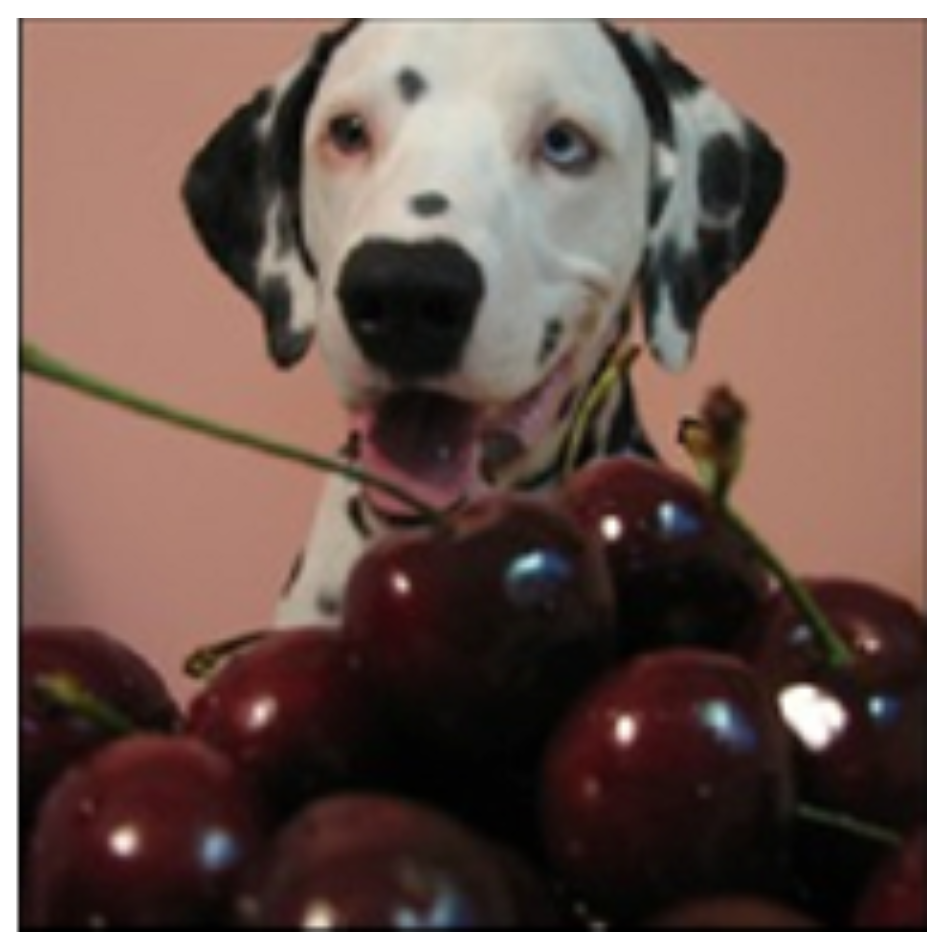
\includegraphics[width=.3\linewidth]{dog_vish.png}
\end{center}
\vfill %
\footnotesize
Можно попробовать сразиться с компьютером:  {\color{blue} \url{https://cs.stanford.edu/people/karpathy/ilsvrc/}}
\end{frame}


\begin{frame}{Точность сетей на ImageNet (Top-5 error rate)}
\begin{center}
	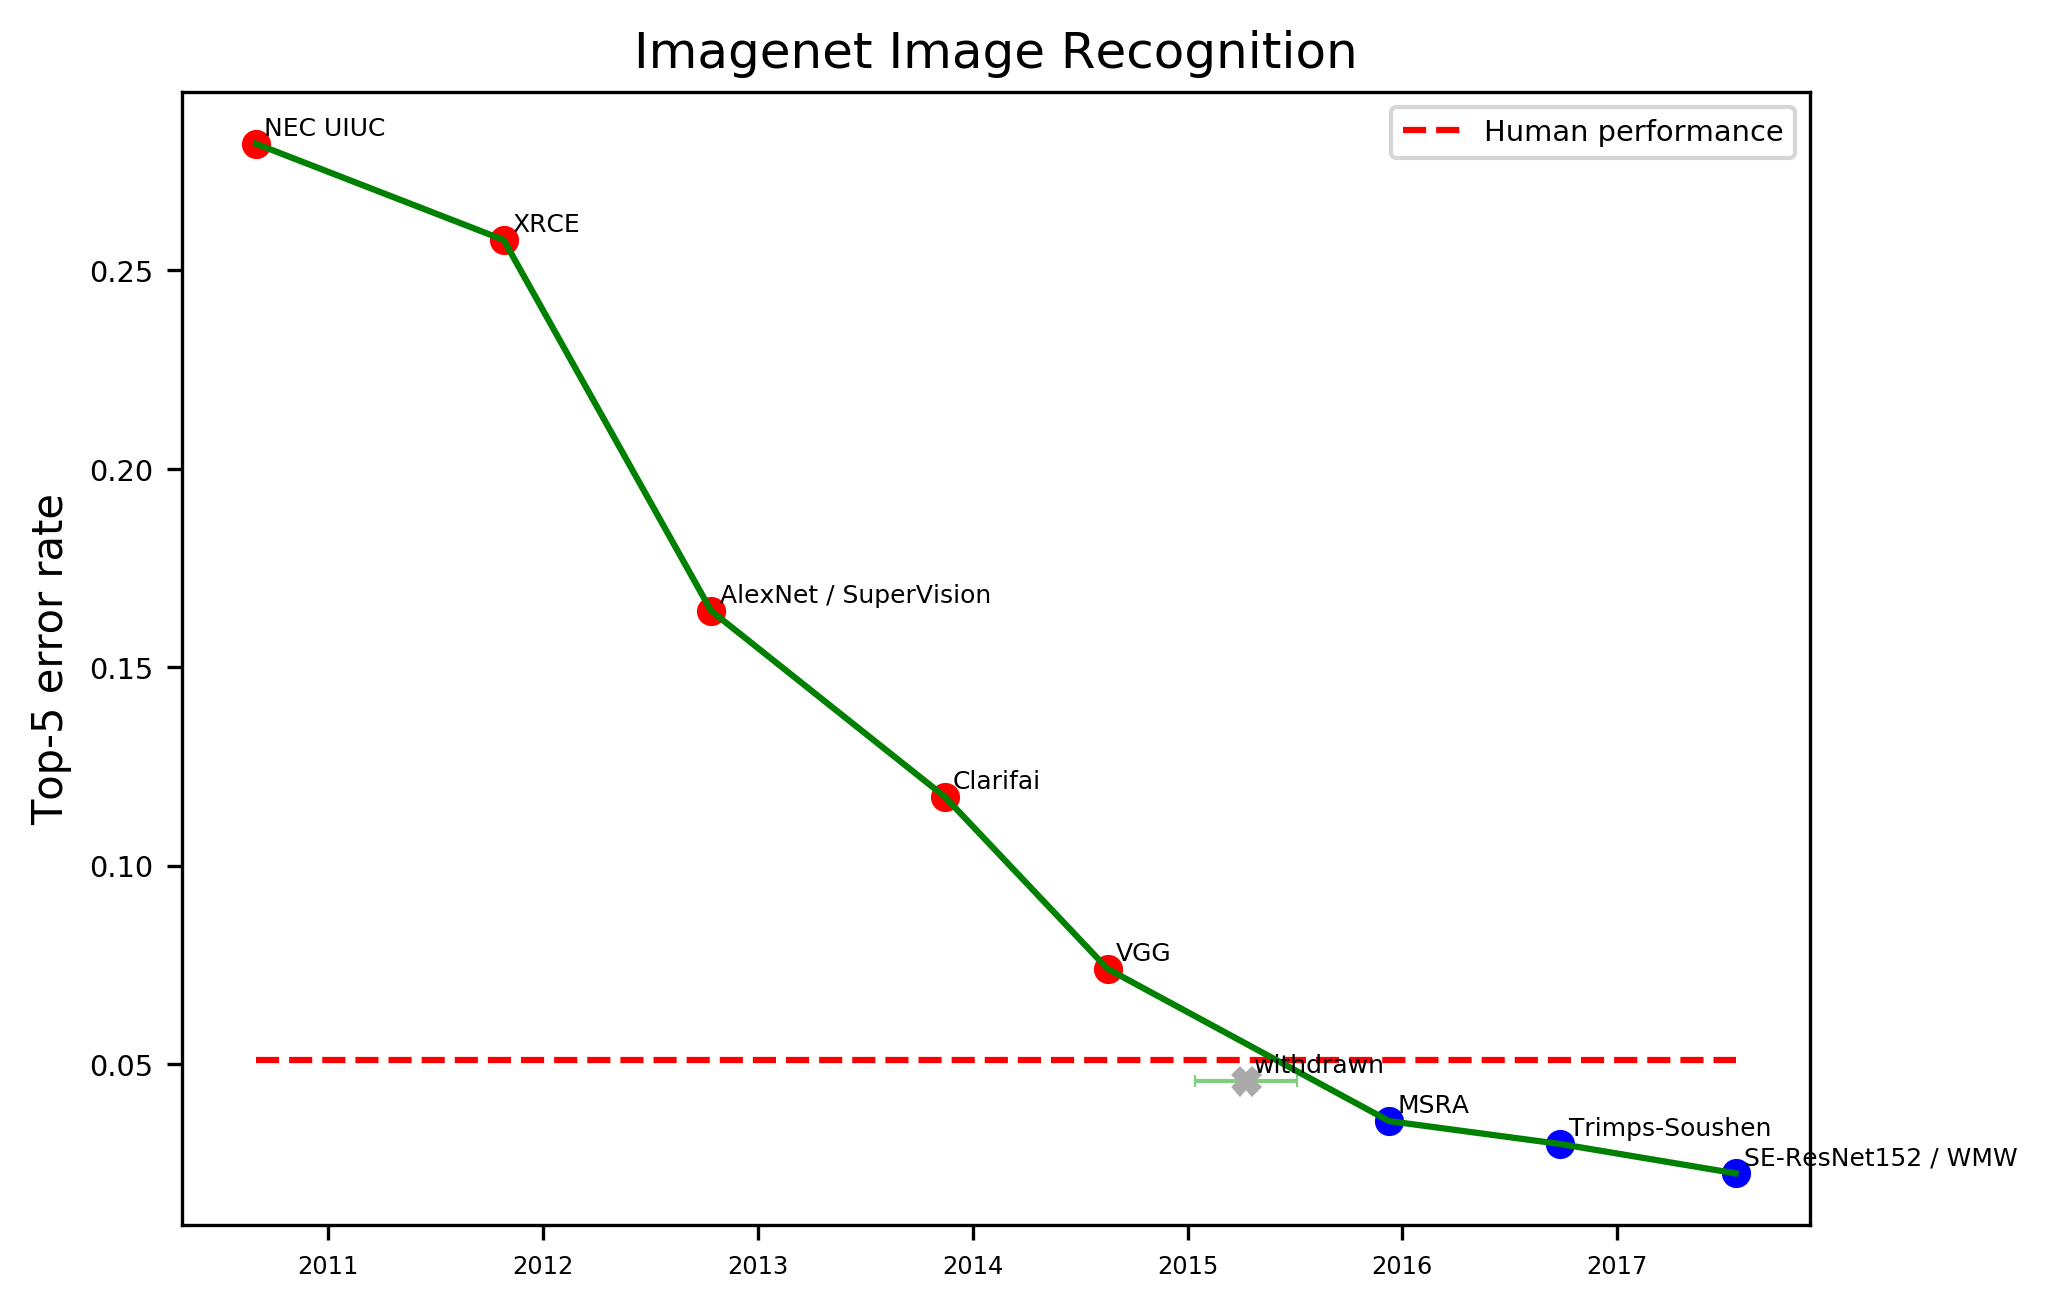
\includegraphics[width=.7\linewidth]{imagenet_recognition.png}
\end{center}
\vfill %
\footnotesize
\color{blue} \url{https://www.eff.org/ai/metrics}
\end{frame} 


\begin{frame}{Точность сетей на ImageNet (Top-1 accuracy)}
\begin{center}
	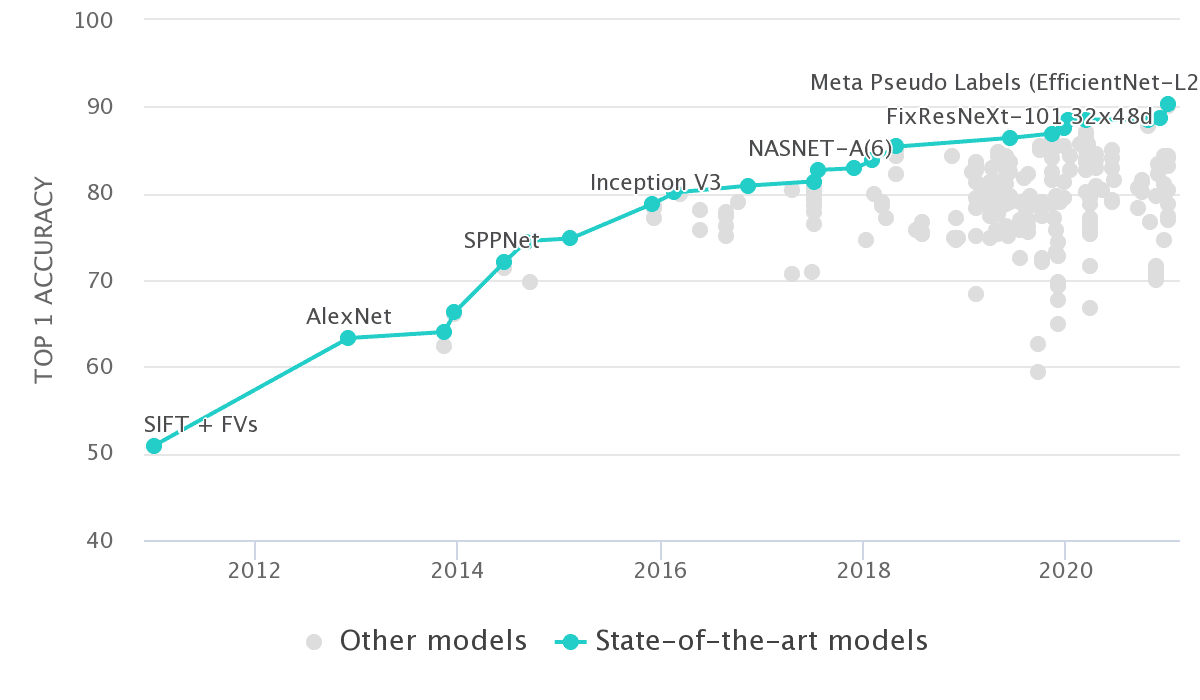
\includegraphics[width=.8\linewidth]{top1_image.png}
\end{center}
\vfill %
\footnotesize
\color{blue} \url{https://theaisummer.com/cnn-architectures/}
\end{frame} 


\begin{transitionframe}
	\begin{center}
		\Huge  AlexNet 
	\end{center}
% \centering 
\includegraphics[scale = 0.6]{jary_alexnet.jpg}
\centering 
\includegraphics[scale = 0.15]{alexnet_jary.png}
\end{transitionframe}


\begin{frame}{AlexNet (2012)}
\begin{center}
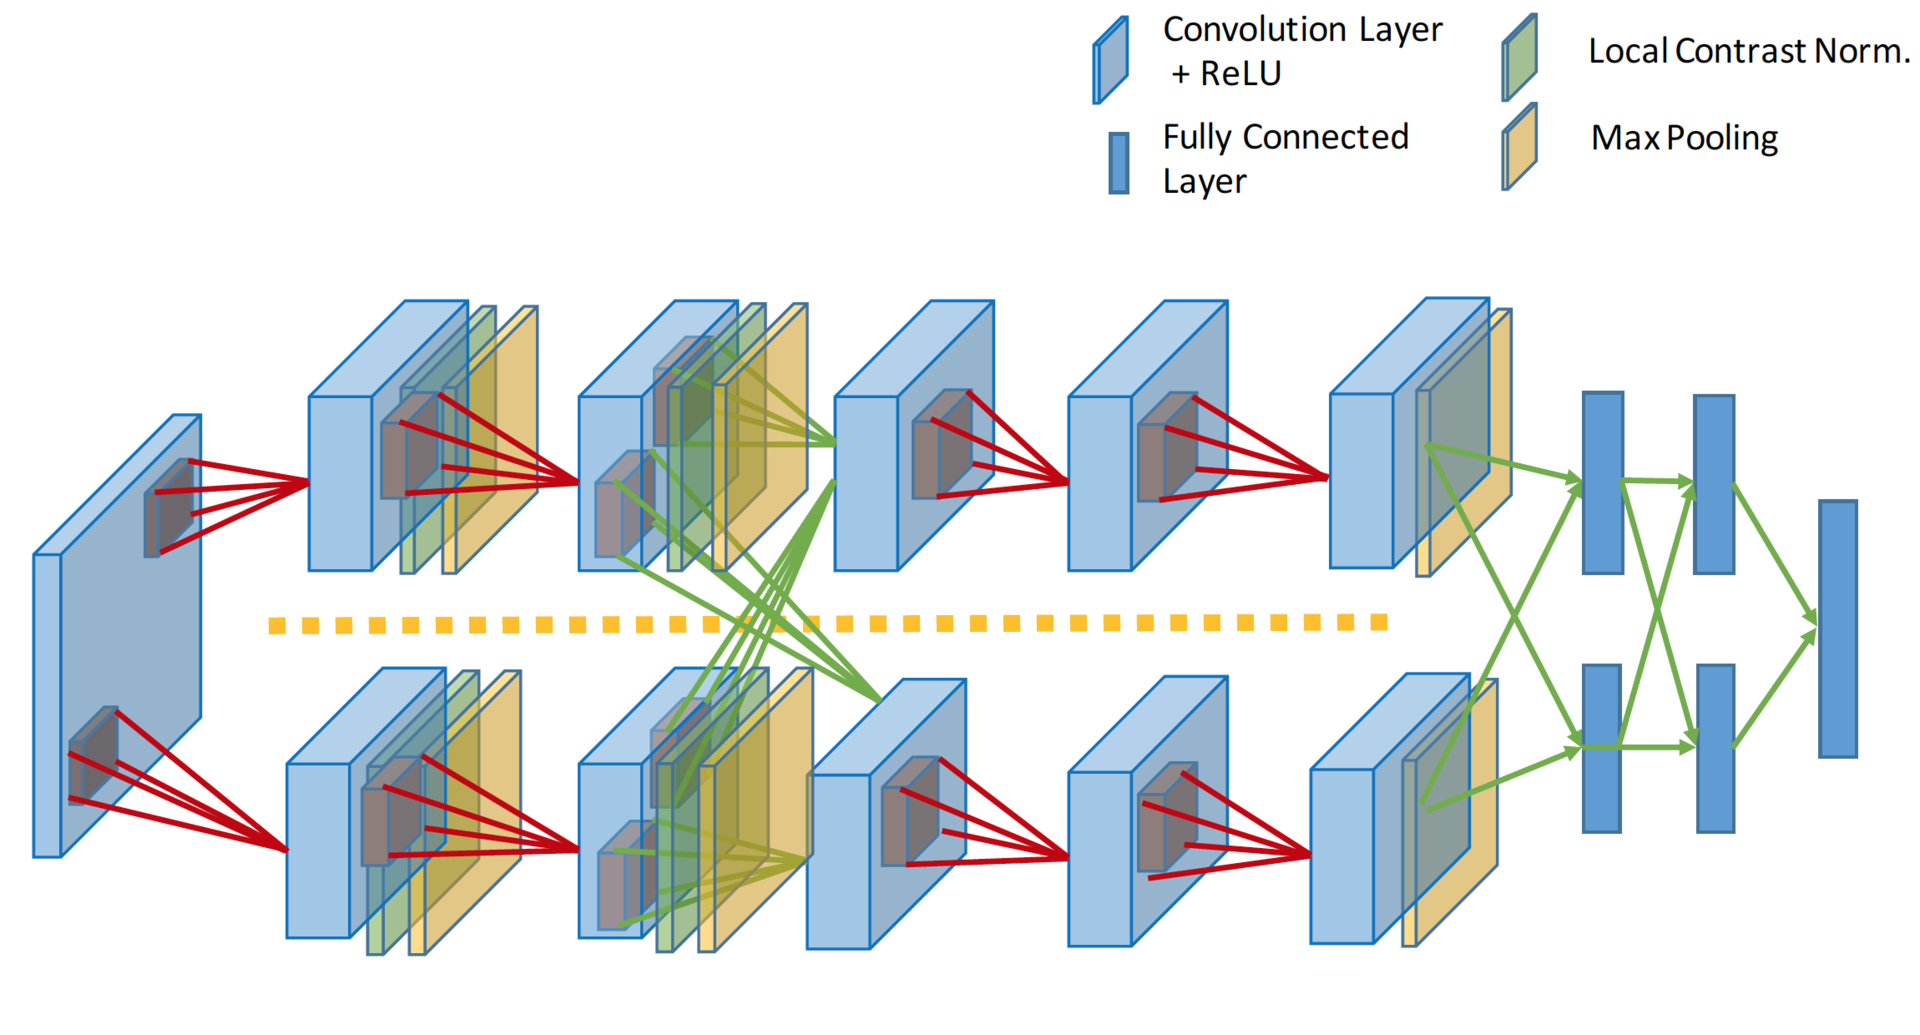
\includegraphics[width=.86\linewidth]{alexnet.png}
\end{center}
\vfill %
\scriptsize
\color{blue} \url{https://papers.nips.cc/paper/4824-imagenet-classification-with-deep-convolutional-neural-networks.pdf}
\end{frame}


\begin{frame}{AlexNet (Krizhevsky et al, 2012)}
\begin{wideitemize}
	\item Использовали ReLU, Dropout, кастомную нормализацию~(не~батчнорм), аугментацию
	\item Использовался градиентный спуск  с инерцией (momentum), размер батча $128$, изначальная скорость обучения $1e-2$, делилась руками на $10$, когда точность на валидации выходила на плато 
	\item Свёртки $11 \times 11$, $5 \times 5$, $3 \times 3$
	\item Около $60$ миллионов параметров, училась $5-6$ суток на $2$ GPU 
	\item Уронила ошибку с $26\%$ до $16.4\%$ 
	\item В $2013$ Zeiler и Fergus потюнили гиперпараметры AlexNet и уронили ошибку до $11.7\%$ (ZFNet)
\end{wideitemize}
\end{frame}


\begin{frame}{Аугментация (Data augmentation)}
	\begin{columns}[T] %
			\begin{column}{.5\textwidth}
					\begin{wideitemize}
							\item Увеличение, уменьшение
							\item Повороты, искажения, приближения
							\item Новые цвета, затемнения
							\item Смена стиля
							\item Нужно ли добавлять сдвиги?  \only<2>{\alert{(нет, вместо них лучше пулинг)} }
						\end{wideitemize}
				\end{column}%
			\hfill%
			\begin{column}{.5\textwidth}
					\begin{center}
							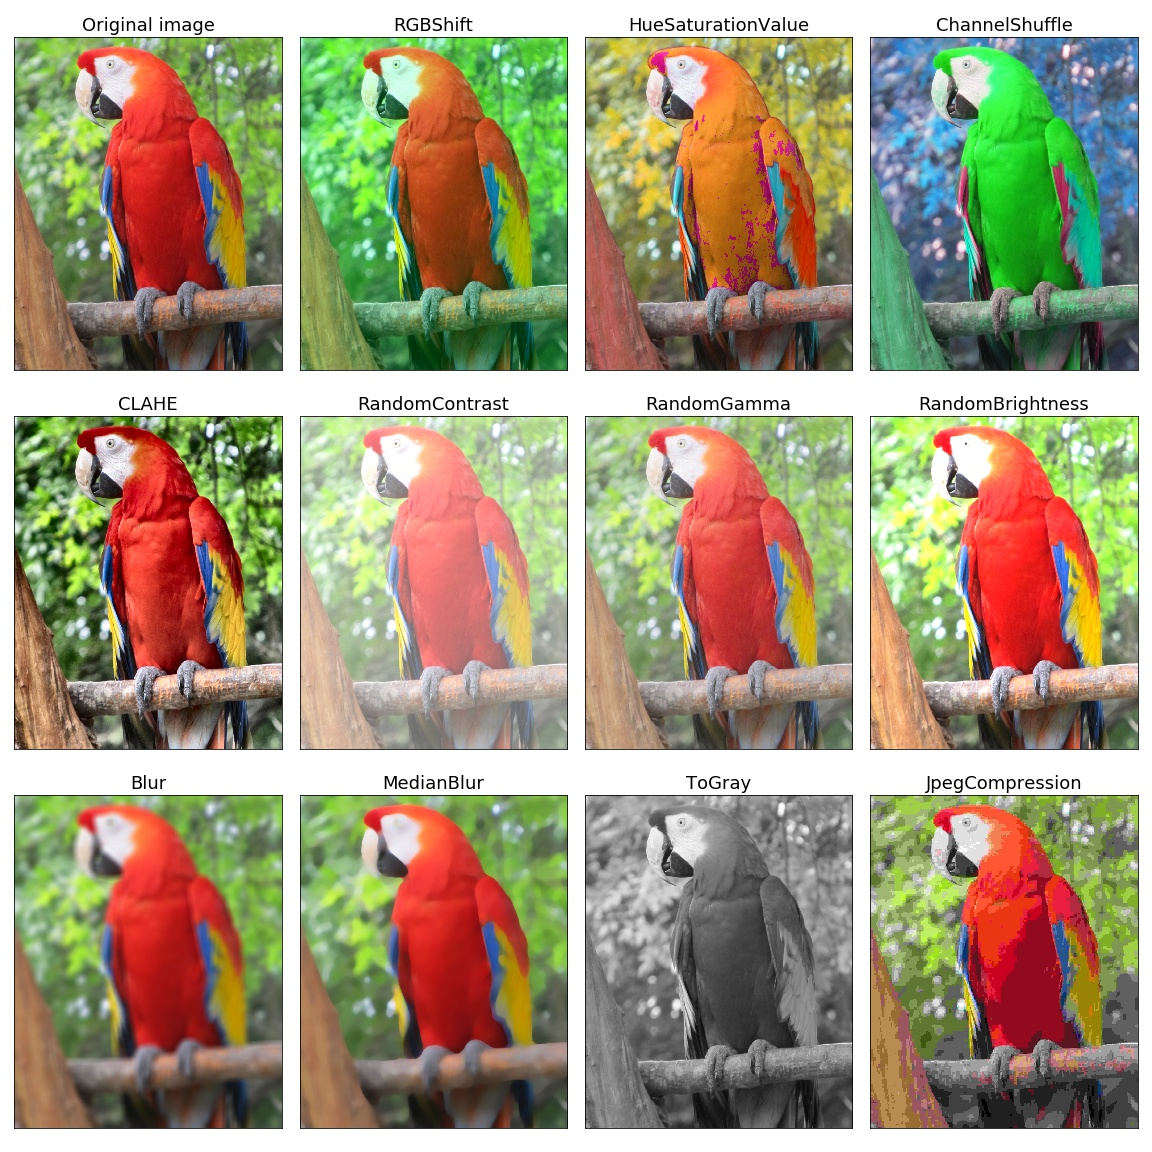
\includegraphics[width=.85\linewidth]{parrot.jpeg}
						\end{center}
				\end{column}%
		\end{columns}
	\vfill
	\footnotesize
	{\color{blue} \url{https://www.tensorflow.org/tutorials/images/data_augmentation}}
\end{frame}


\begin{frame}{Аугментация (Data augmentation)}
	\begin{wideitemize}
			\item Много разных вариантов
			\item «Бесплатное» расширение обучающей выборки
			\item \alert{Обучение:}  случайно применяем к картинкам из текущего батча
			\item \alert{Тест:} делаем несколько аугментаций картинки, применяем сеть к каждой и усредняем предсказания
			\item Для тестовых данных набор аугментаций всегда фиксирован 
		\end{wideitemize}
\end{frame}

\begin{frame}{ ImageNet augmentations}
	\begin{center}
		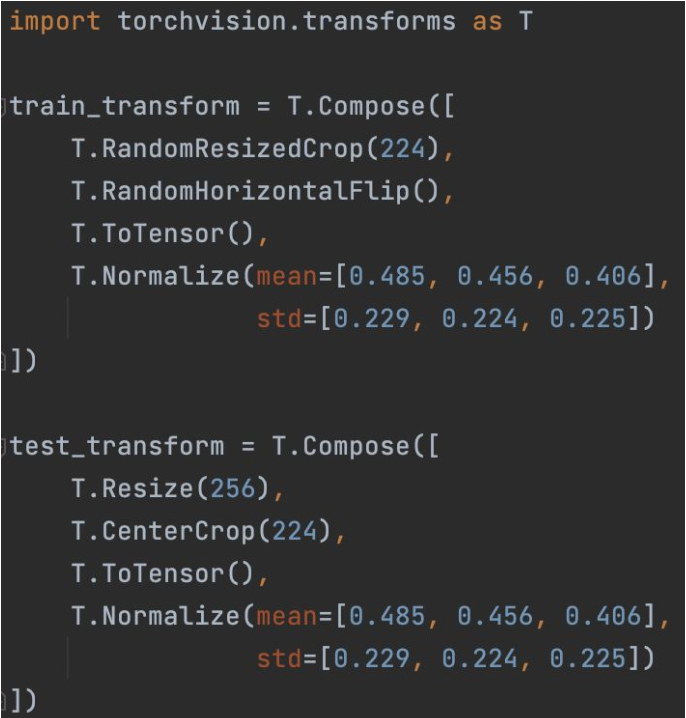
\includegraphics[width=.45\linewidth]{imgnet_aug.png}
	\end{center}
\end{frame}


 \begin{transitionframe}
	\begin{center}
		\Huge  Visual Geometry Group (VGG)
	\end{center}
\centering 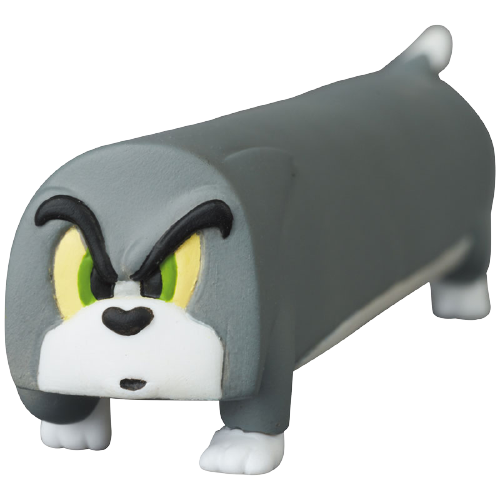
\includegraphics[scale = 0.25]{vgg_tom.png}
\end{transitionframe}

\begin{frame}{VGG (2014)}
\begin{center}
	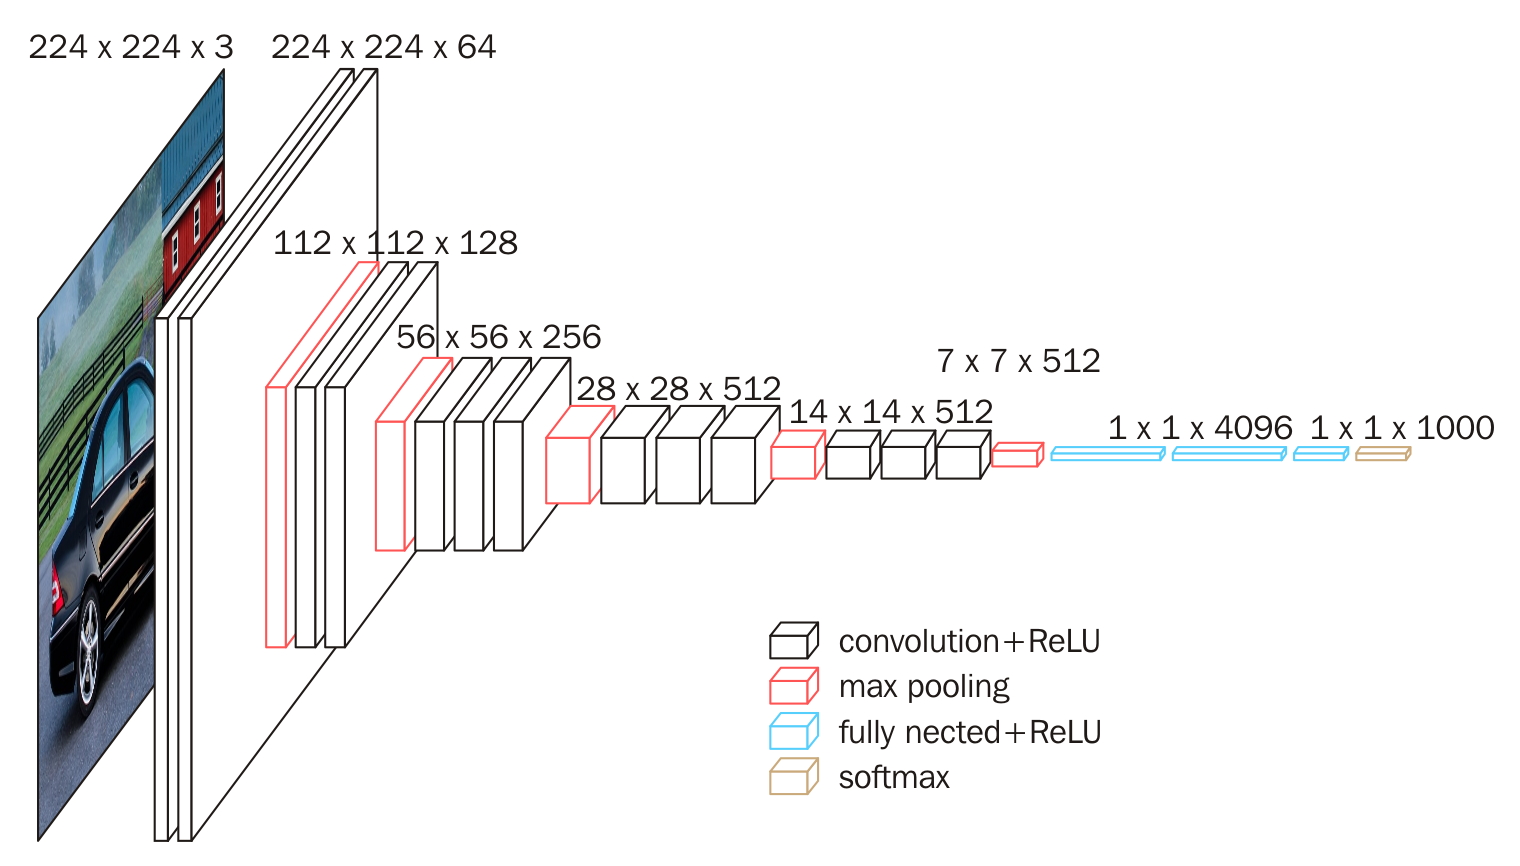
\includegraphics[width=.7\linewidth]{vgg.png}
\end{center}
\vfill %
\footnotesize
\color{blue} \url{h8ps://arxiv.org/pdf/1409.1556.pdf}
\end{frame}

\begin{frame}{VGG (2014)}
\begin{wideitemize}
	\item Свёртки только $3 \times 3$, но намного больше фильтров 
	\item Экономия параметров (две свёртки $3\times 3$ покрывают поле $5 \times 5$ и требуют $18$ параметров, а свёртка $5 \times 5$ требует $25$ параметров)
	\item Дропаут для первых двух полносвязных слоёв, Momentum, хитрая инициализация
\end{wideitemize}

\begin{columns}[T] % align columns
	\begin{column}{.58\textwidth}
		\begin{wideitemize}	
			\item  $138$ миллионов параметров, училась $2-3$ недели на $4$ GPU 
			\item Ошибка упала до $7\%$
		\end{wideitemize}
	\end{column}%
	\hfill%
	\begin{column}{.38\textwidth}
		\begin{center}
			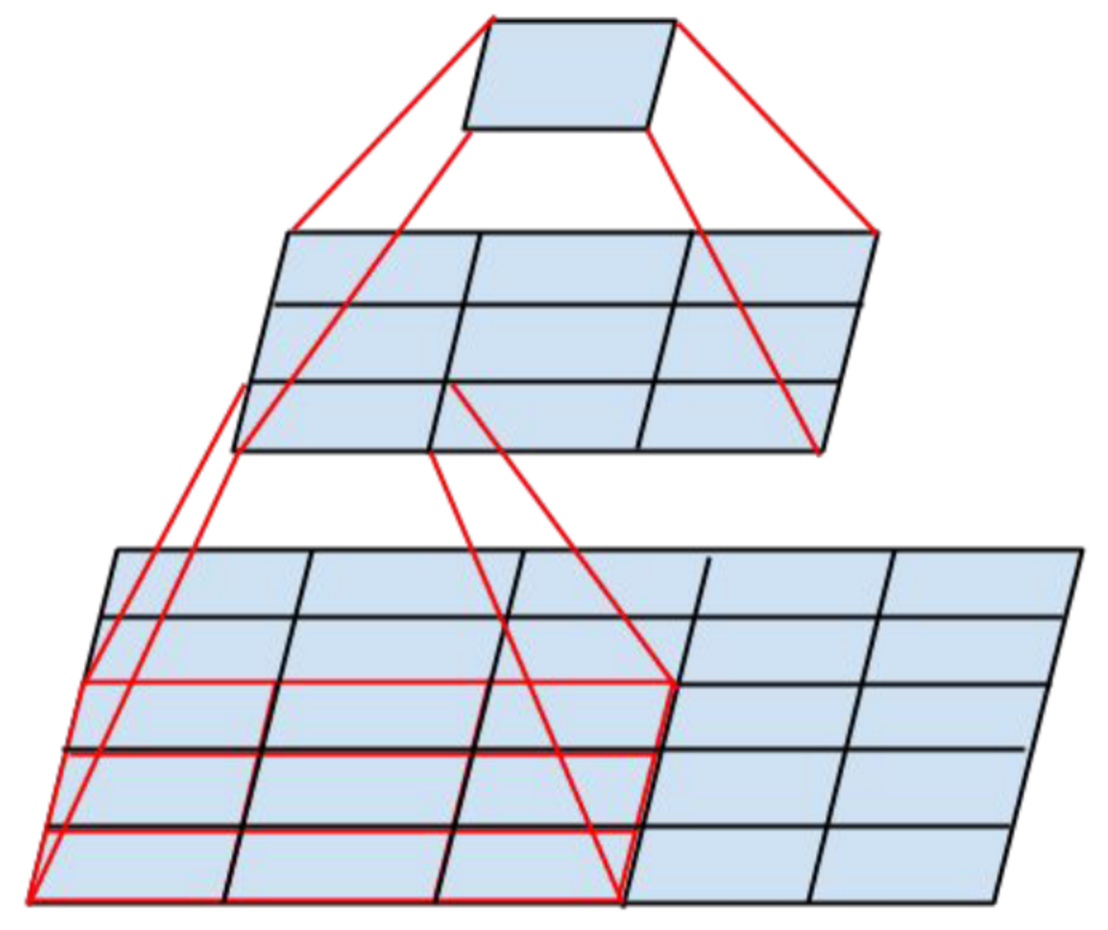
\includegraphics[width=.6\linewidth]{vgg_conv.png}
		\end{center}
	\end{column}%
\end{columns}
\end{frame}


 \begin{transitionframe}
	\begin{center}
		\Huge  GoogleLeNet aka Inception
	\end{center}
\centering 
\includegraphics[scale = 0.25]{googleNet_top.png}
\end{transitionframe}


\begin{frame}{GoogleLeNet aka Inception V1}
\begin{center}
	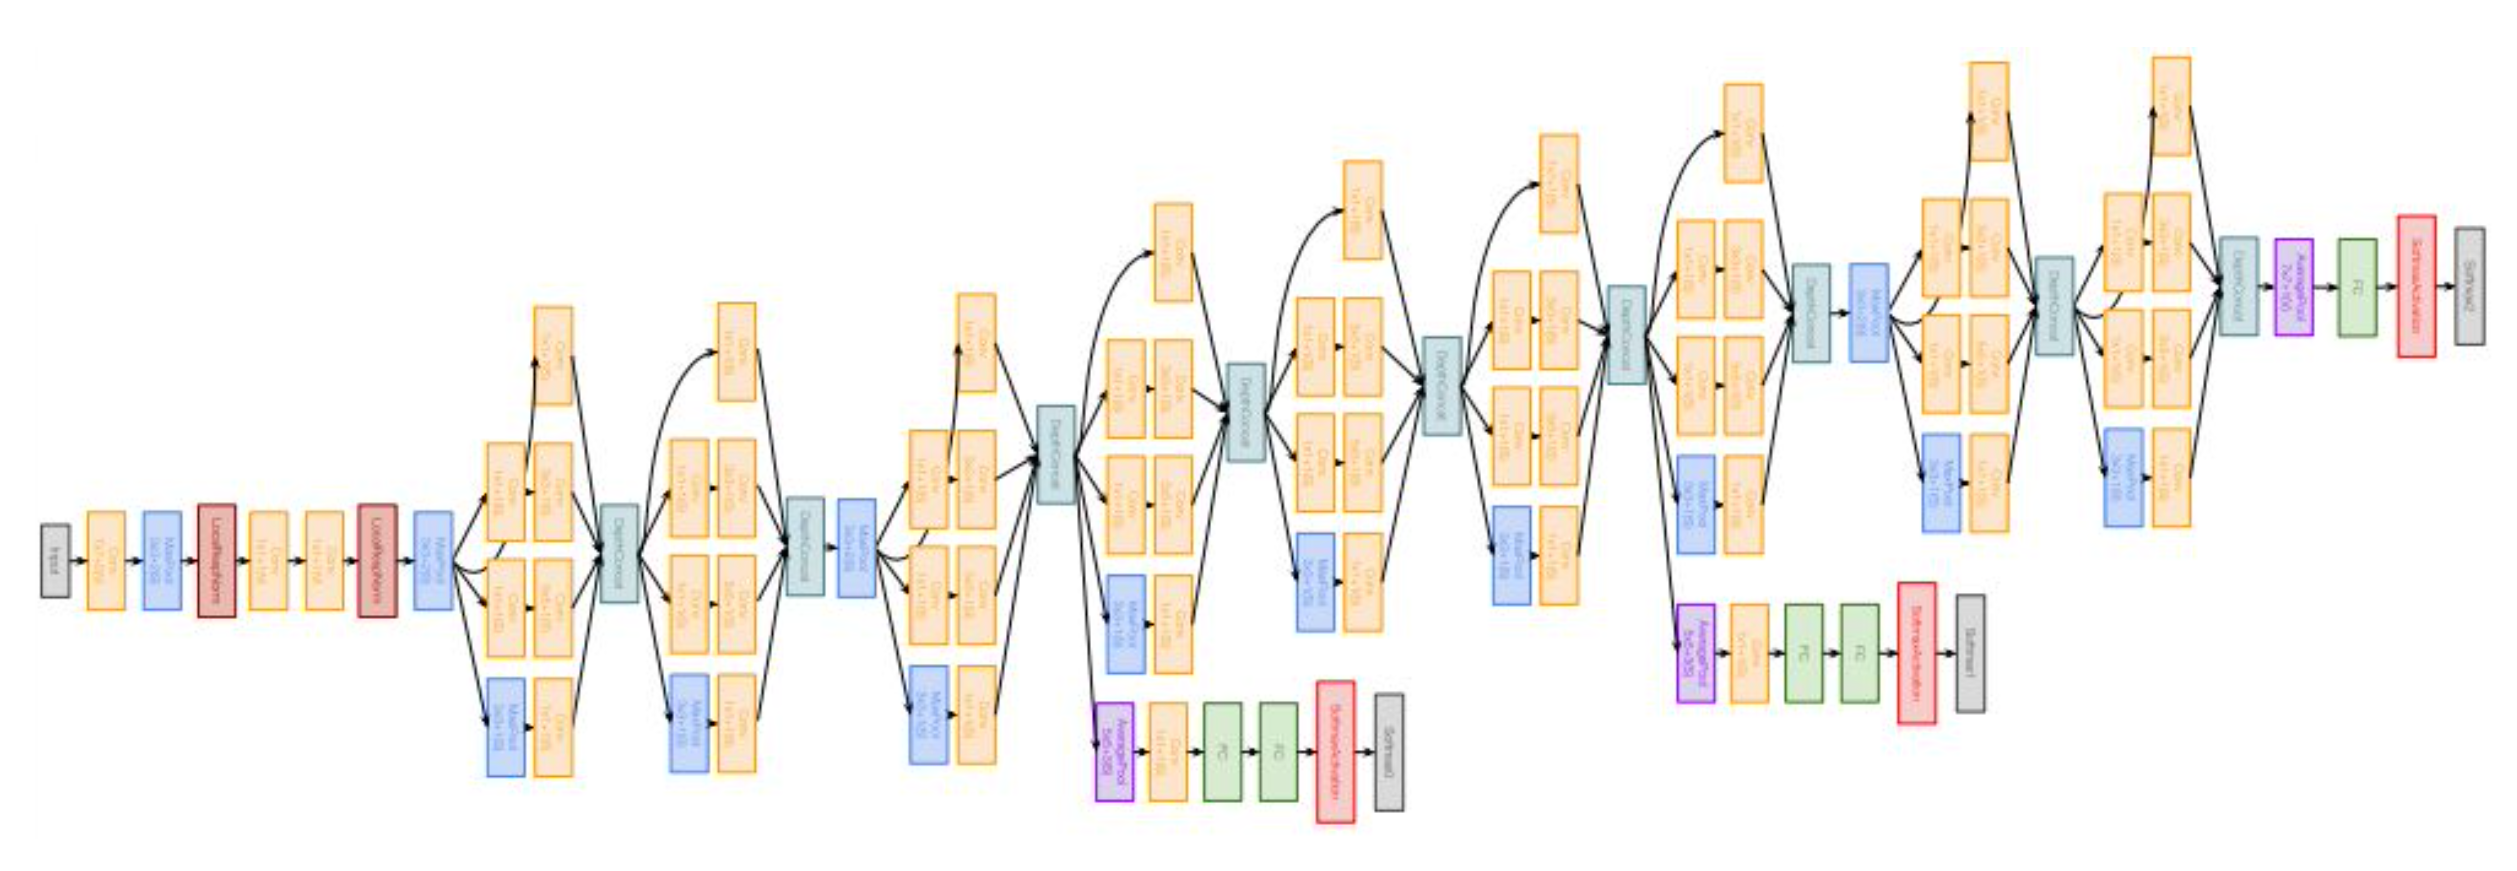
\includegraphics[width=.99\linewidth]{stanford_lenet.png}%{inception.png}
\end{center}
\vfill %
\footnotesize
\color{blue} \url{https://arxiv.org/abs/1409.4842}
\end{frame}


\begin{frame}{GoogleLeNet aka Inception V1  (2014)}
\begin{wideitemize}
	\item  Уменьшаем свёртки, саму \alert{сетку собираем из специальных inception-блоков}  (9 блоков)
		
	\item используются  \alert{свёртки $1 \times 1$} для уменьшения числа каналов перед "тяжёлыми" свёртками 
	
	\item \alert{Несколько дополнительных классификаторов на разных уровнях,} идея в том, что такие классификаторы позволят «протолкнуть» градиенты к ранним слоям и тем самым уменьшить эффект затухания градиента
	
	\item  Параметров  в $10$ раз меньше, чем в AlexNet, ошибка упала до $6.7\%$
\end{wideitemize}
\end{frame}


\begin{frame}{Свёртка $1 \times 1$}
\begin{columns}[T] %
	\begin{column}{.4\textwidth}
		\begin{wideitemize}
			\item  Позволяет сократить размерность по числу каналов
			\item  Представляет из себя полносвязный слой по фильтрам 
			\item  В Inception мы делаем много разных свёрток, а потом свёрткой $1 \times 1$ выбираем из них лучшее, агрессивно понижая размерность
		\end{wideitemize}
	\end{column}%
	\hfill%
	\begin{column}{.6\textwidth}
		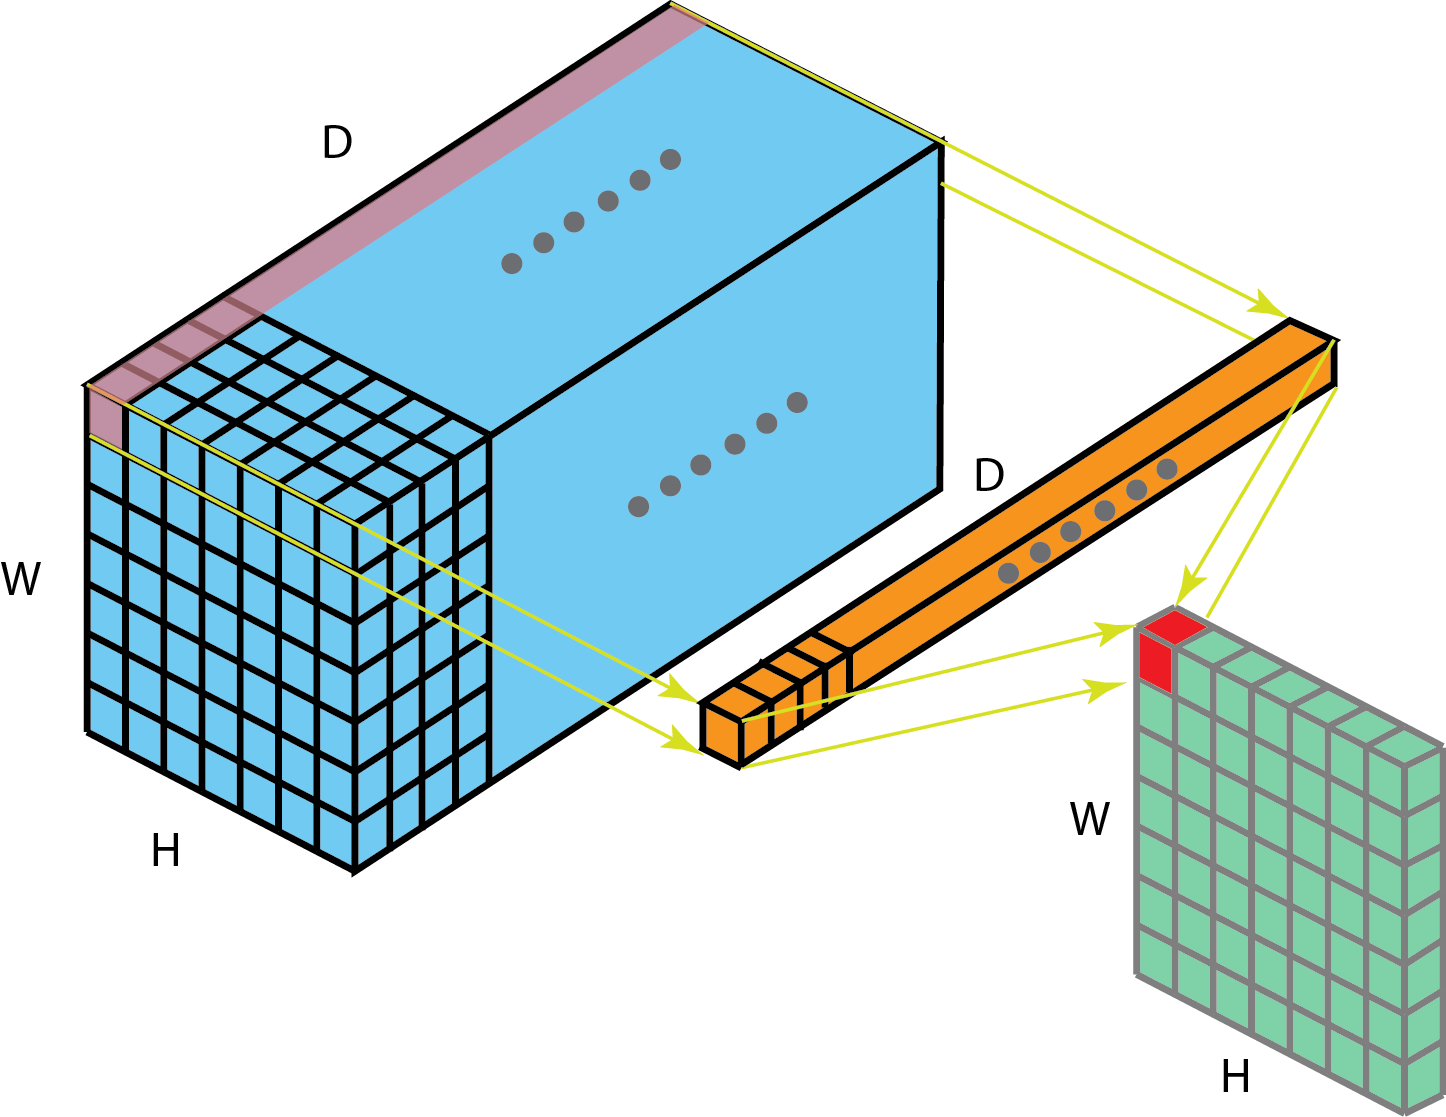
\includegraphics[width=.9\linewidth]{11conv.png}
	\end{column}%
\end{columns}
\end{frame}


\begin{frame}{GoogleLeNet aka Inception V1  (2014)}
\begin{columns}[T] % align columns
	\begin{column}{.4\textwidth}
		\begin{wideitemize}	
			\item  На каждом слое используется ни одна свёртка, а несколько разных, что помогает реагировать на сигналы разного масштаба
			\item Свёртка $1 \times 1$ делает вычисления легче
		\end{wideitemize}
	\end{column}%
	\hfill%
	\begin{column}{.6\textwidth}
		\begin{center}
			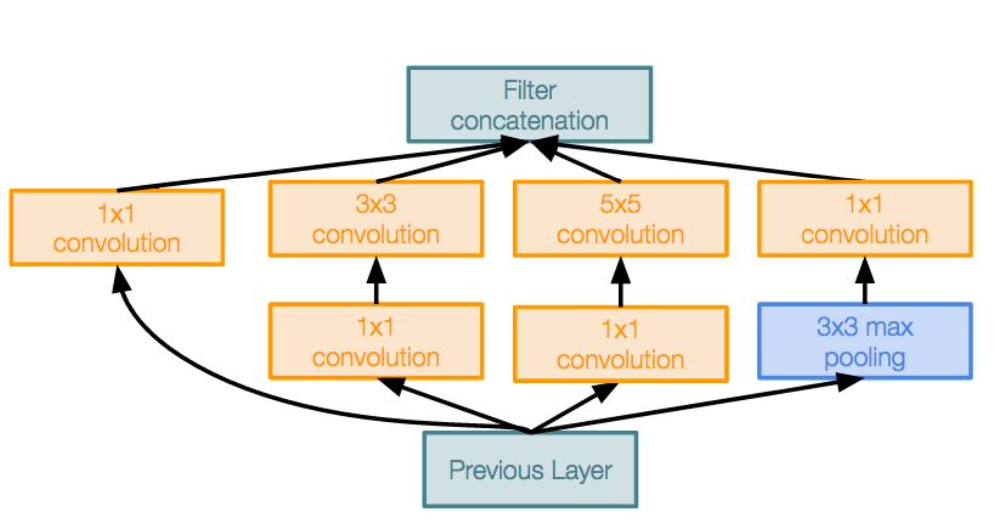
\includegraphics[width=.99\linewidth]{inception_stanford.png}
		\end{center}
	\end{column}%
\end{columns}
\vfill %
\footnotesize
\color{blue} \url{https://arxiv.org/abs/1409.4842}
\end{frame}


\begin{frame}{GoogleLeNet aka Inception V1}
\begin{center}
	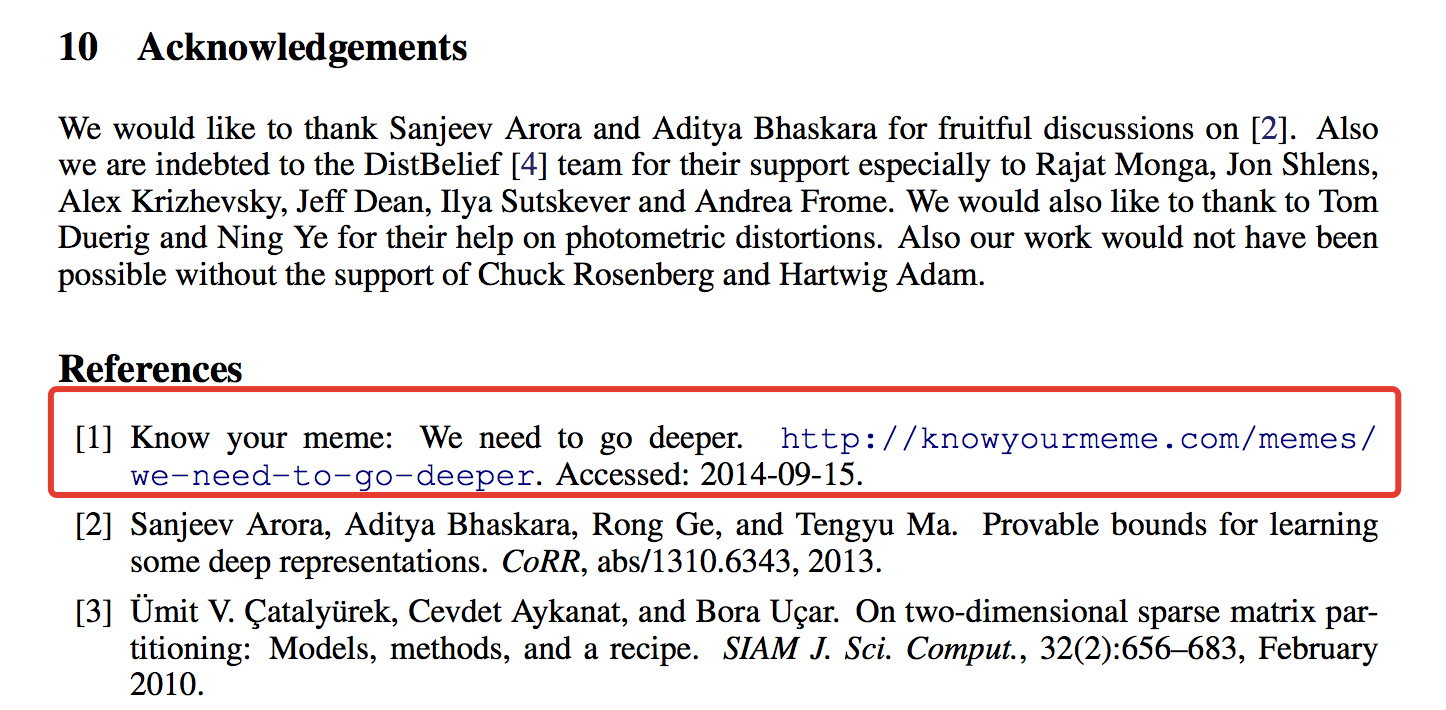
\includegraphics[width=.8\linewidth]{memes_incep.png}
\end{center}
\end{frame}


\begin{frame}{Inception V3 (2015)}
\begin{center}
	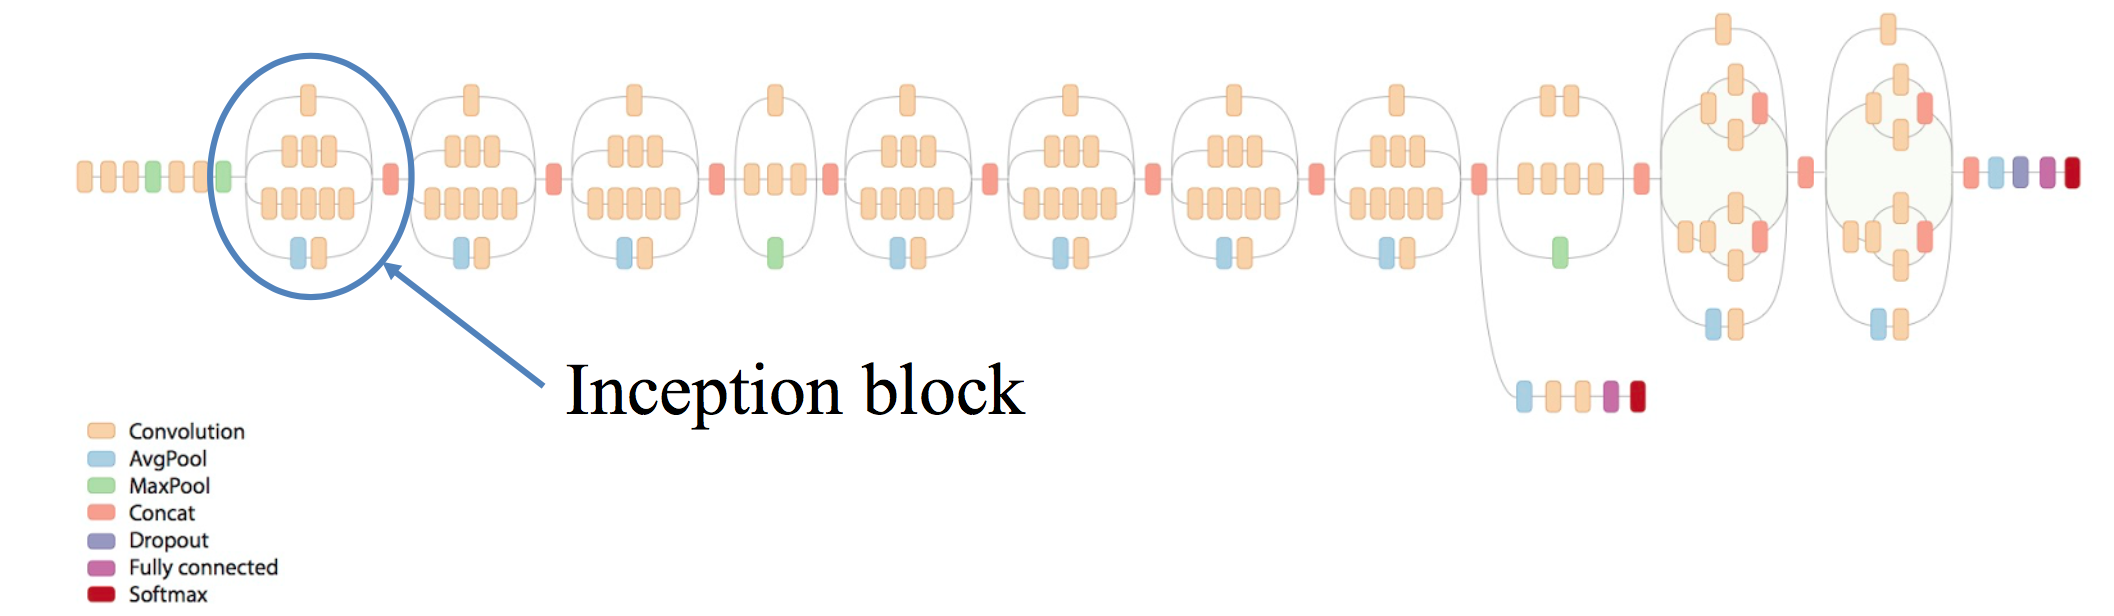
\includegraphics[width=.99\linewidth]{inception3.png}
\end{center}
\vfill %
\footnotesize
\color{blue} \url{https://arxiv.org/abs/1512.00567}
\end{frame}


\begin{frame}{Свёртка $n \times 1$ и $1 \times n$ }
\begin{columns}[T] %
	\begin{column}{.6\textwidth}
	\centering	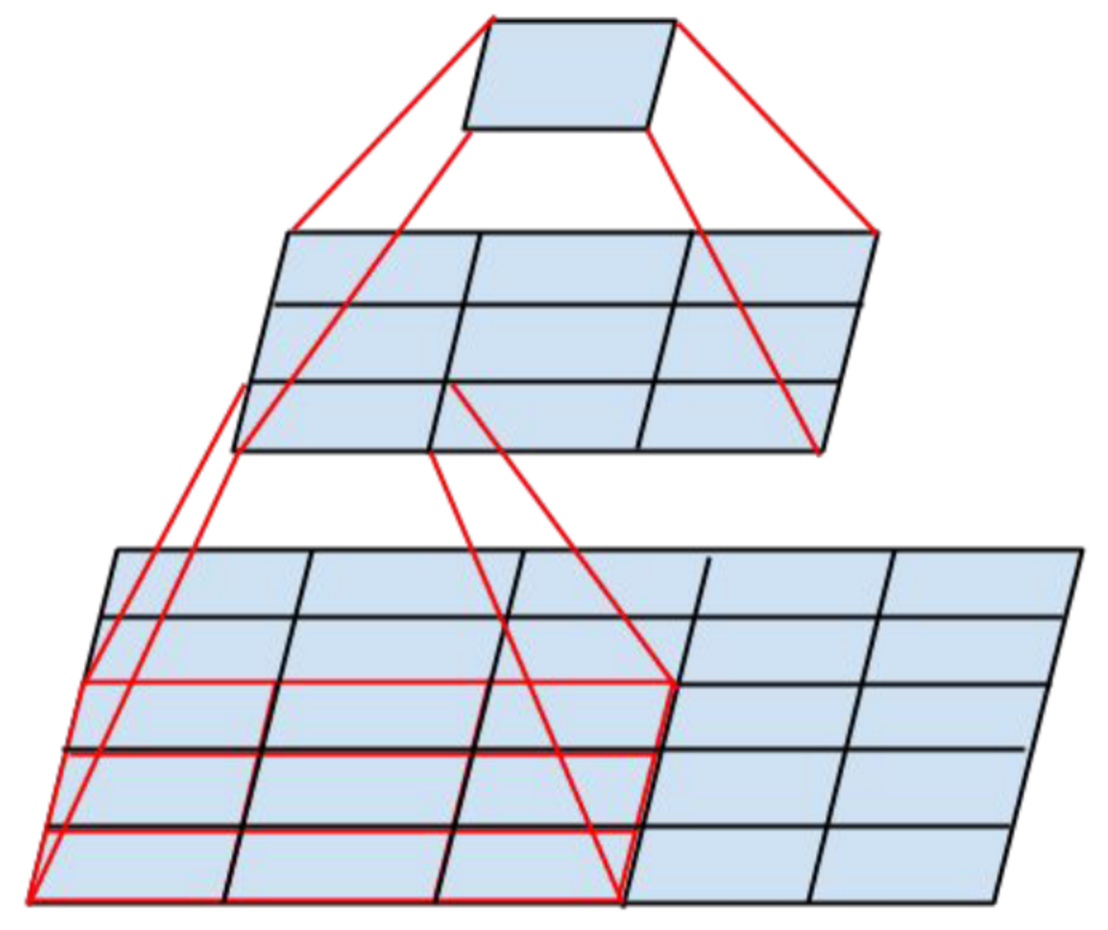
\includegraphics[width=.42\linewidth]{vgg_conv.png}
	\end{column}%
	\hfill%
	\begin{column}{.4\textwidth}
	\centering 	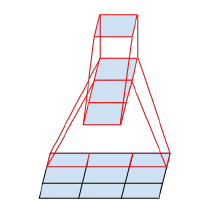
\includegraphics[width=.5\linewidth]{conv_inc_1.png} 
	\end{column}%
\end{columns}
\vfill
\begin{itemize}
	\item В VGG заменяли большие свёртки на последовательные $3 \times 3$
	\item Пойдём дальше и заменим их на последовательные $3 \times 1$ и $1 \times 3$
	\item Экономим ещё больше параметров, для каждой свёртки $6$ вместо $9$ 
\end{itemize}
\end{frame}


\begin{frame}{Inception V3 (2015)}
\begin{center}
	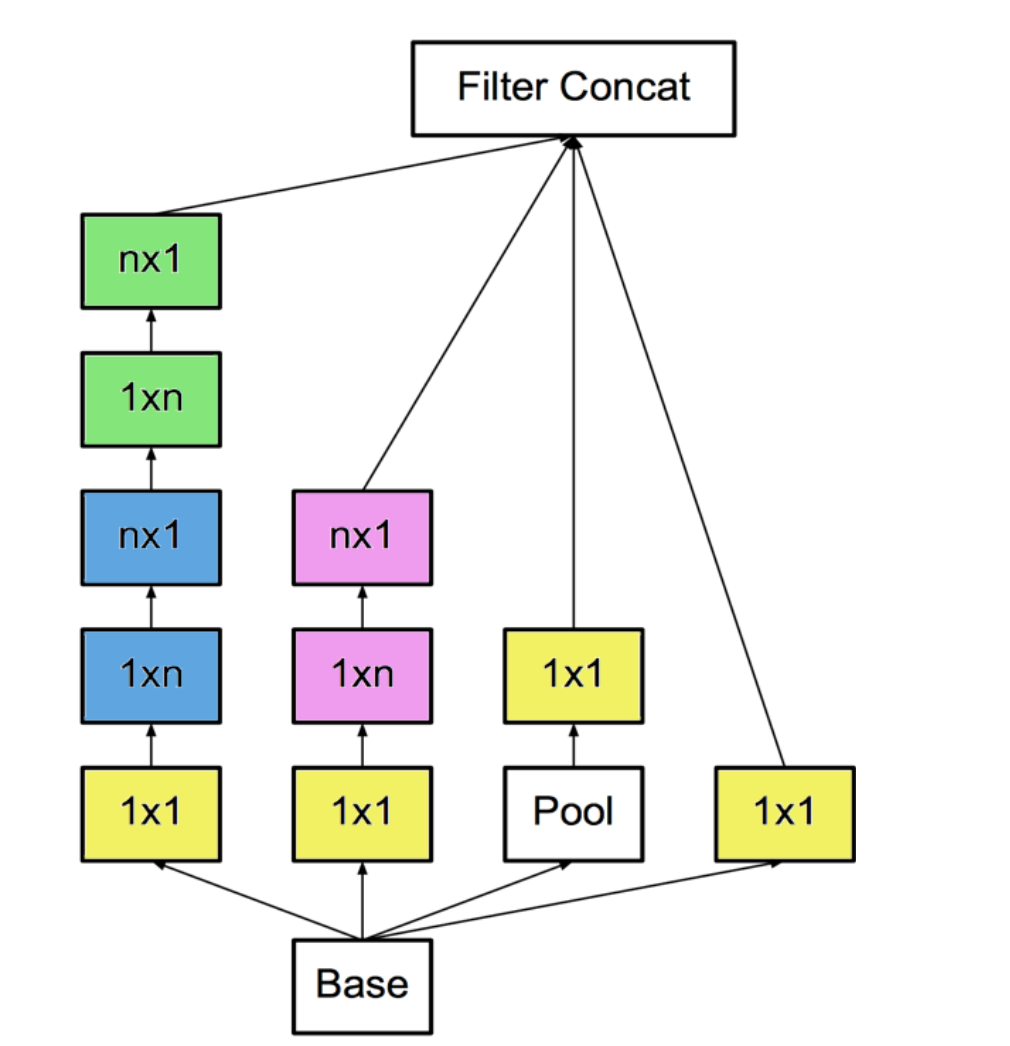
\includegraphics[width=.5\linewidth]{block3.png}
\end{center}
\end{frame}


\begin{frame}{Inception V3 (2015)}
\begin{wideitemize}
	\item  Сетка собирается из $11$ inception layers, добавили BatchNorm (то же самое без него было в Inception V2)
	
	\item В результате исследований сформулировали \alert{принципы обучения глубоких свёрточных сетей:}
	
	\begin{enumerate}
		\item  Избегайте representation bottlenecks, нельзя резко снижать размерность слоя, это надо делать плавно: от начала к концу
		\item Свёртку нужно разбивать на более мелкие части для экономии ресурсов и увеличения размера сетки 
		\item Нельзя резко увеличивать глубину, забивая на ширину, надо растить сбалансированно
	\end{enumerate} 

	\item Итоговое качество $4.2\%$ ошибок, ансамбль из $4$-х моделей дал $3.8\%$. 
\end{wideitemize}
\end{frame}


 \begin{transitionframe}
	\begin{center}
		\Huge  ResNet
	\end{center}
\end{transitionframe}



\begin{frame}{ResNet (Microsoft) (2015)}
\begin{center}
	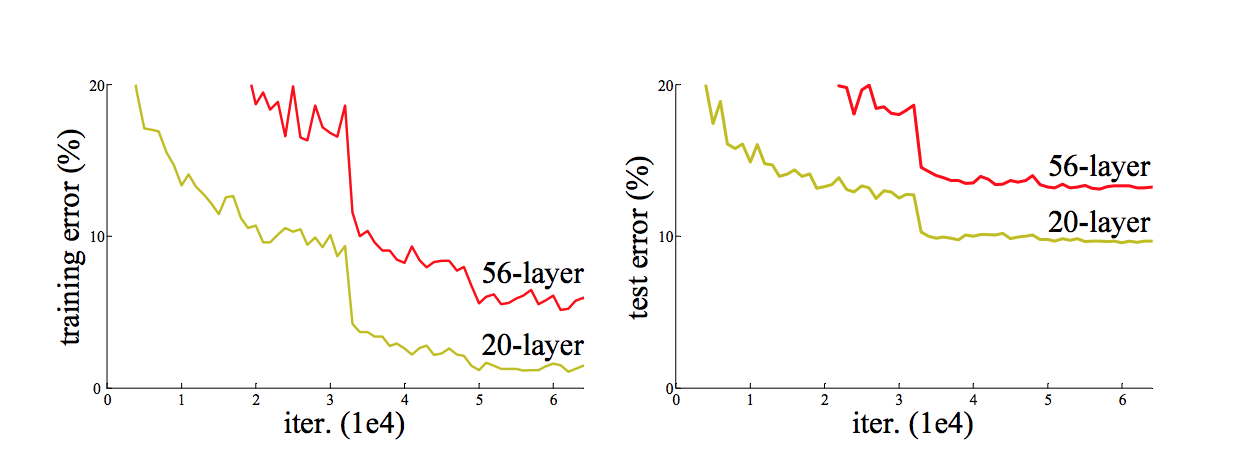
\includegraphics[scale=0.35]{resnet_idea.png}
\end{center}
\vfill %
\footnotesize
\color{blue} \url{https://arxiv.org/abs/1512.03385}
\end{frame}


\begin{frame}{ResNet (Microsoft) (2015)}
\begin{wideitemize}
	\item  Добавление слоёв в свёрточную сеть ухудшает качество даже на обучении
	\item  Хотя возможностей для переобучения больше, сеть почему-то не может ими воспользоваться
	\item  \alert{Интерпретация эффекта:} слои инициализированы шумом, если какой-то один слой не натренирован, он убивает работу сети, через него не проходит полезный сигнал 
	\item Чем больше слоёв, тем более ярко выражен этот эффект 
\end{wideitemize}
\end{frame}


\begin{frame}{ResNet (Microsoft) (2015)}
\begin{wideitemize}
	\item \alert{Решение проблемы:} Будем посылать вход на выход и давать слою возможность немного его подправить (residual слой)
	\item Идея чем-то похожа на бустинг, сеть сама решает когда заканчивать подправлять выходы (грубо говоря, сама выбирает глубину)
\end{wideitemize}
\end{frame}


\begin{frame}{ResNet (Microsoft) (2015)}
\begin{center}
	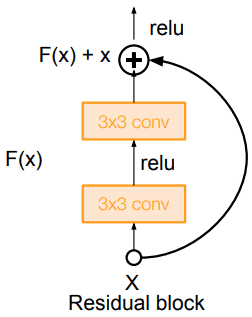
\includegraphics[scale=0.6]{resnet_layer.png}
\end{center}
\vfill %
\footnotesize
\color{blue} \url{https://arxiv.org/abs/1512.03385}
\end{frame}


\begin{frame}{Residual Block }
	\begin{center}
		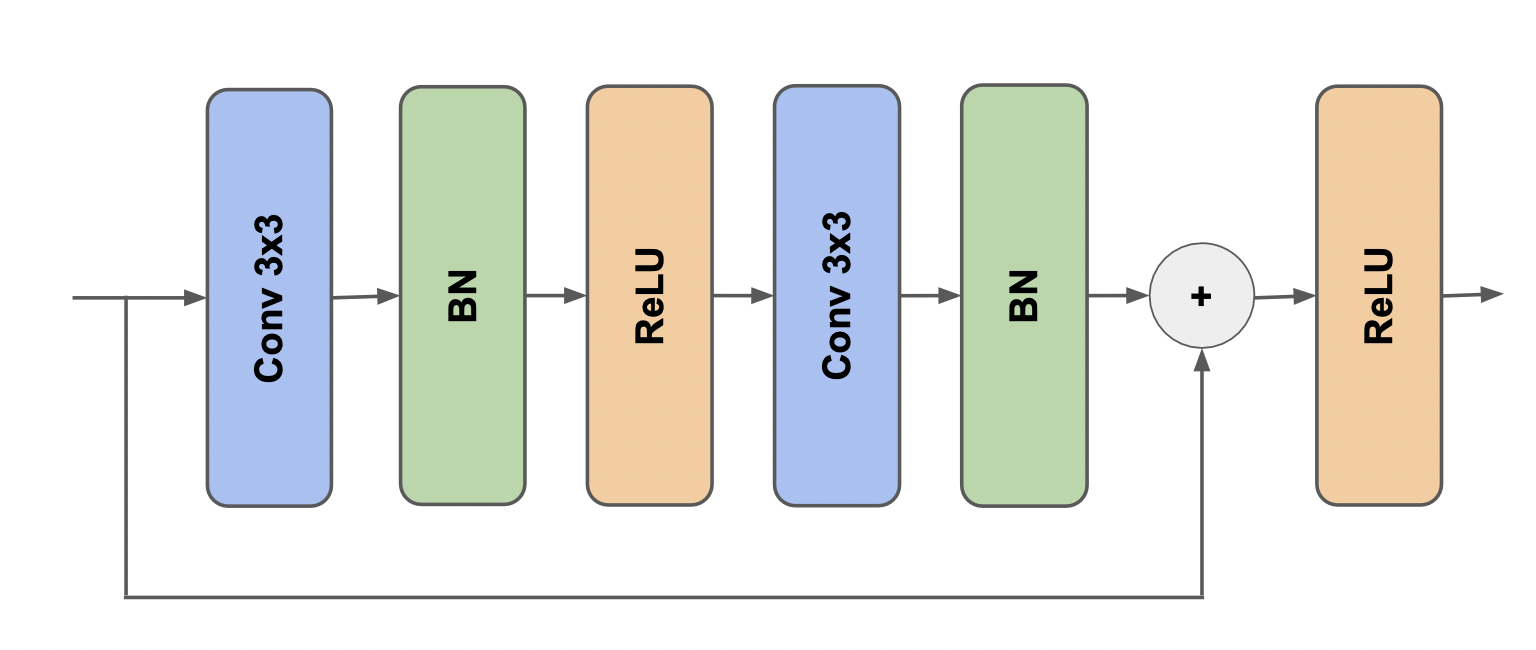
\includegraphics[scale=0.5]{residual_block.png}
	\end{center}
	\vfill %
	\footnotesize
	\color{blue} \url{https://arxiv.org/abs/1512.03385}
\end{frame}


\begin{frame}{ResNet (Microsoft) (2015)}
\begin{center}
	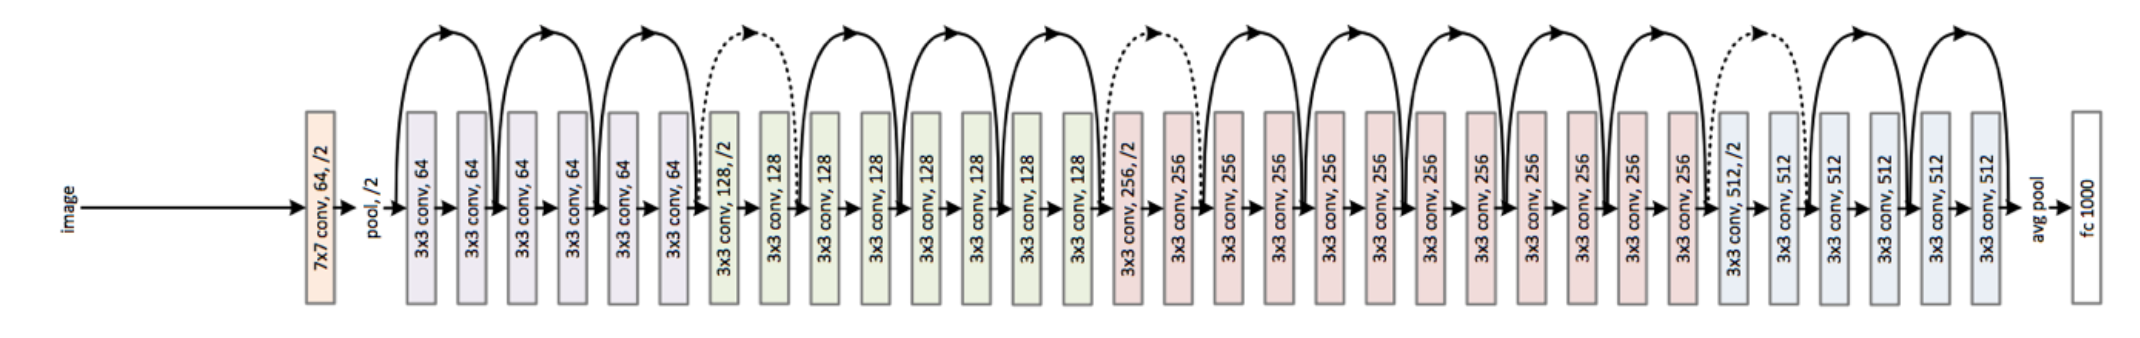
\includegraphics[scale=0.2]{resnet.png}
\end{center}
\begin{itemize}
	\item 152 слоя, ошибка составила $3.6\%$
\end{itemize}
\vfill %
\footnotesize
\color{blue} \url{https://arxiv.org/abs/1512.03385}
\end{frame}


\begin{frame}{ResNet (Microsoft) (2015)}
\begin{wideitemize}
	\item \alert{Идея:} более глубокие уровни должны улавливать разницу между новым и тем, что было раньше 
	
	\item Ключевым элементом архитектуры является связь, которая пропускает несколько слоёв, передавая результат предыдущего слоя
	
	\item Используется инициализация Ксавье, батч нормализация после каждого свёрточного слоя
	
	\item Обучение с помощью Momentum SGD, cтартовая скорость $0.1$, уменьшается в $10$ раз при выходе ошибки на тесте на плато, размер батча $256$
\end{wideitemize}
\vfill %
\footnotesize
\color{blue} \url{https://arxiv.org/abs/1512.03385}
\end{frame}


\begin{frame}{ResNet (Microsoft) (2015)}
\begin{center}
	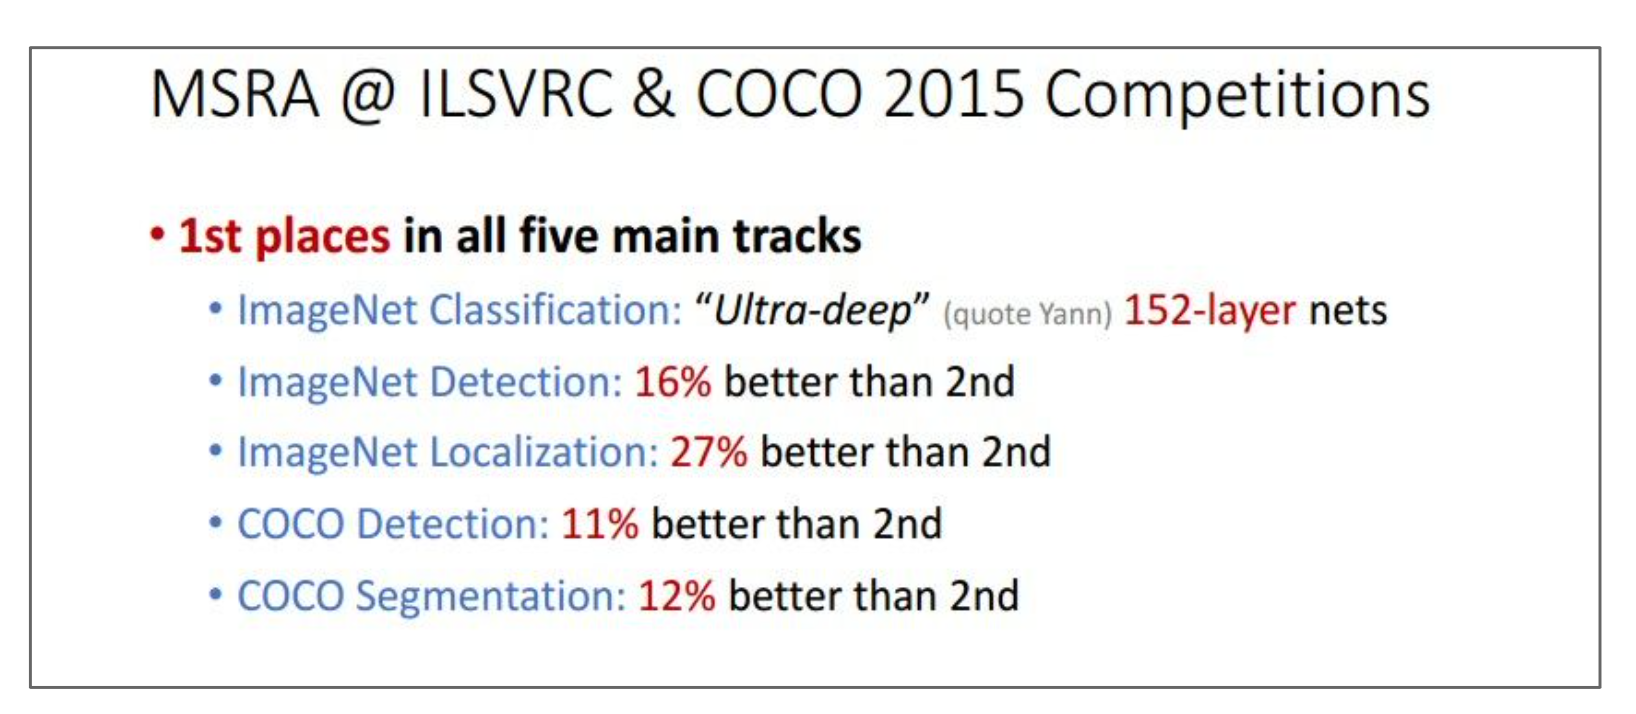
\includegraphics[width=.8\linewidth]{winner_2015.png}
\end{center}
\vfill %
\footnotesize
\color{blue} \url{https://arxiv.org/abs/1512.03385}
\end{frame}


\begin{frame}{Why  skip-connections ?}
	\begin{center}
		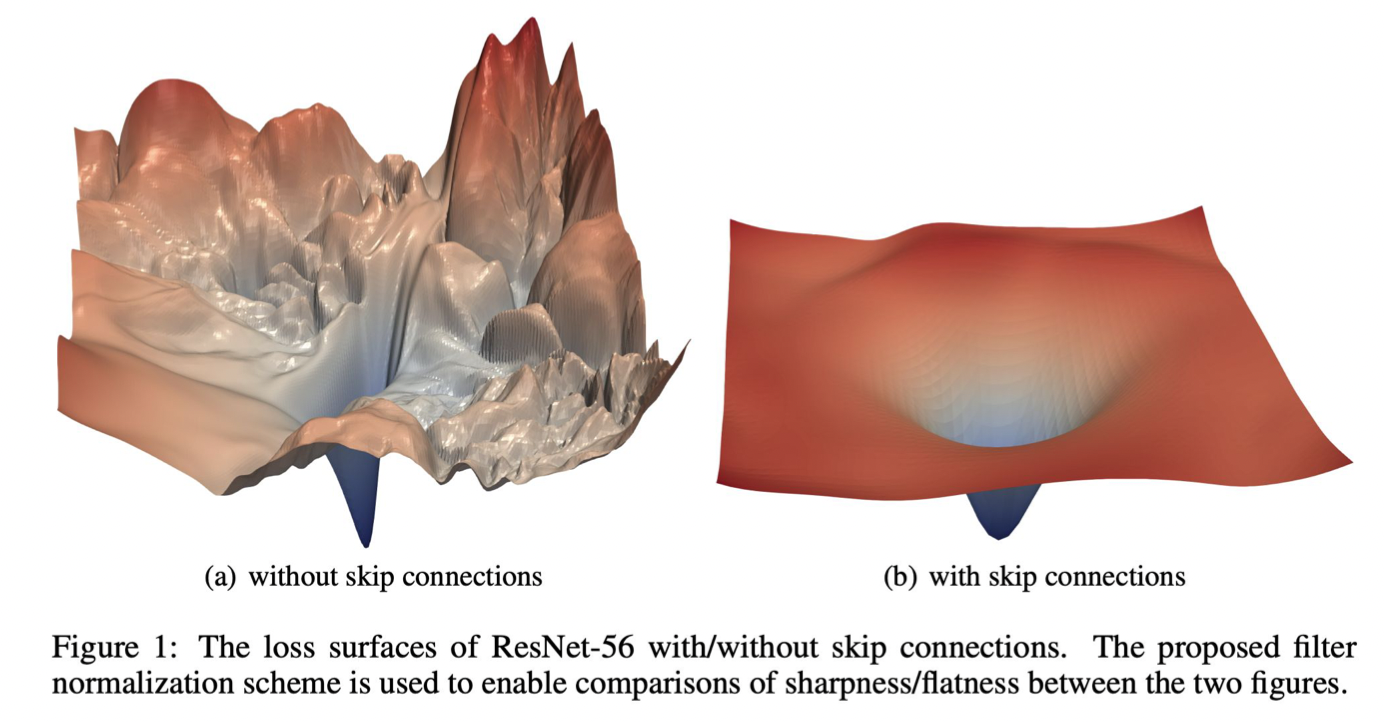
\includegraphics[width=.8\linewidth]{skip-conn_land.png}
	\end{center}
	\vfill %
	\footnotesize
	\color{blue} \url{https://arxiv.org/abs/1712.09913}
\end{frame}


 \begin{transitionframe}
	\begin{center}
		\Huge  Что было дальше? 
	\end{center}
\centering 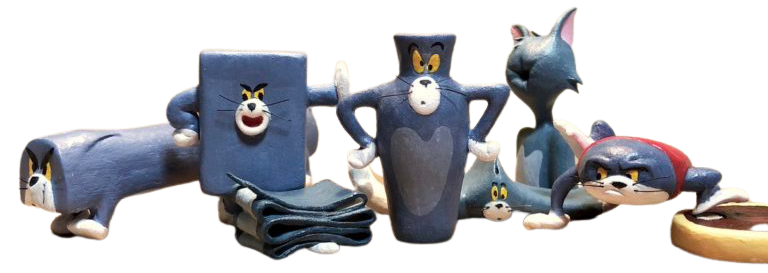
\includegraphics[scale = 0.35]{next_steps.png}
\end{transitionframe}


\begin{frame}{Inception-Resnet  (2016)}
\begin{columns}[T] %
	\begin{column}{.5\textwidth}
		\begin{wideitemize}
			\item Совместили две идеи вместе
			\item Судя по всему, виды слоёв перебирали автоматически, но не палятся
			\item Ансамблем Google поставил новый рекорд $3.08\%$
		\end{wideitemize} 
	\end{column}%
	\hfill%
	\begin{column}{.5\textwidth}
		\centering 	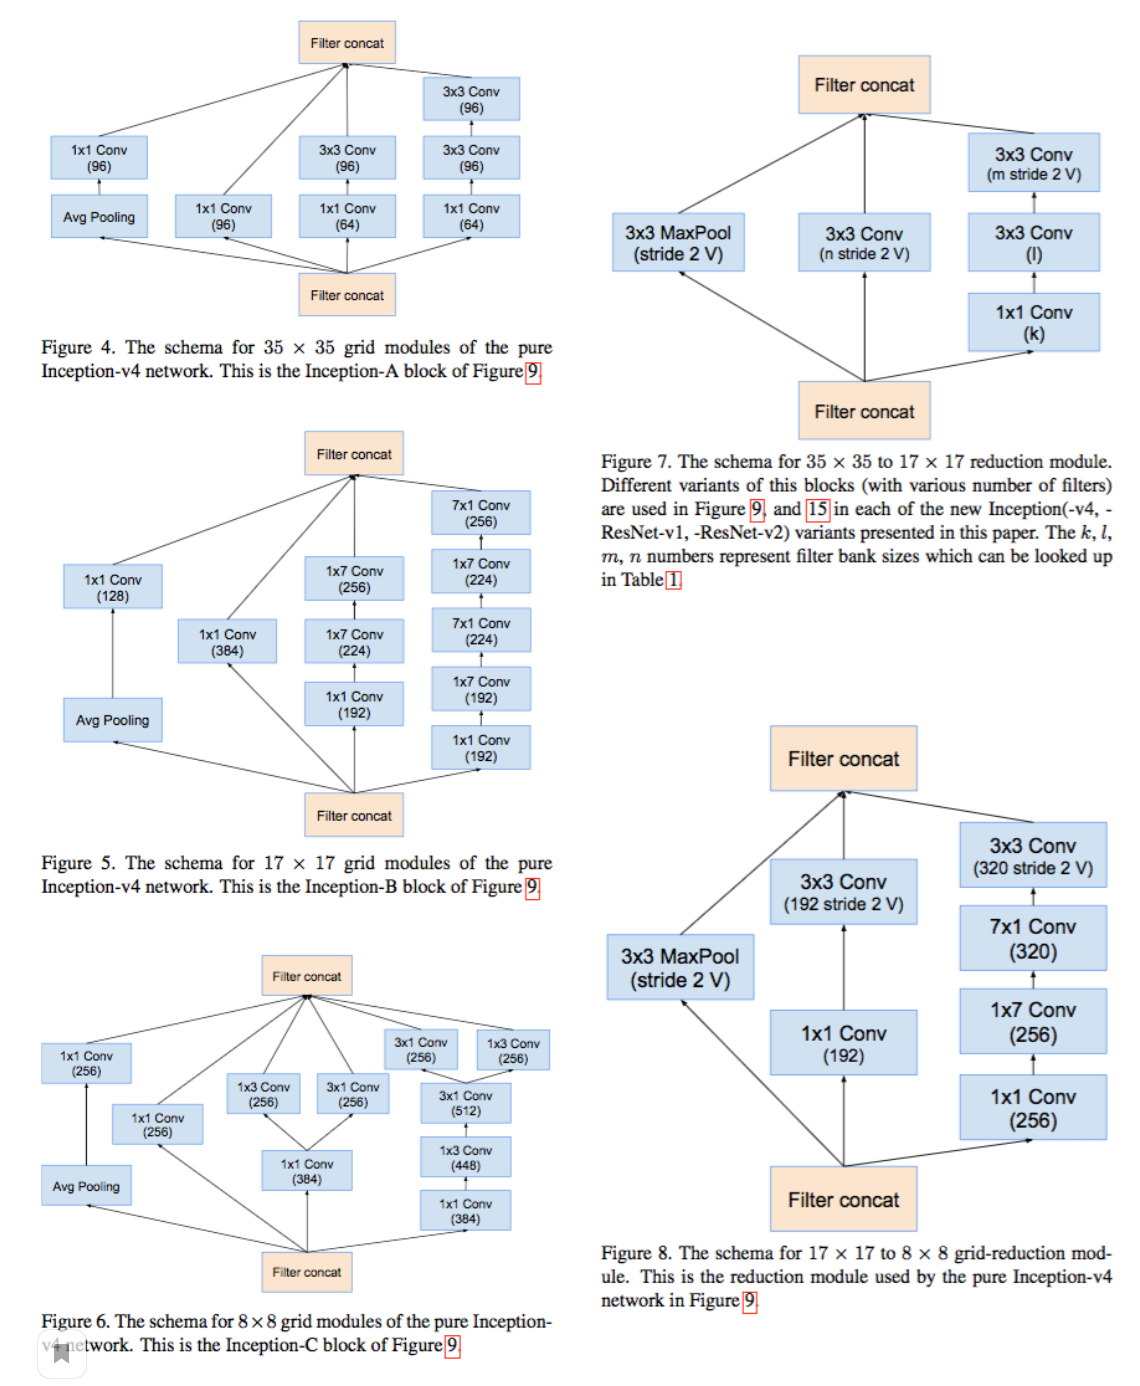
\includegraphics[width=.8\linewidth]{inception_resnet.png} 
	\end{column}%
\end{columns}
\vfill %
\footnotesize
\color{blue} \url{https://arxiv.org/abs/1602.07261}
\end{frame}


\begin{frame}{DenseNet  (2018)}
	\begin{columns}[T] %
		\begin{column}{.5\textwidth}
			\begin{wideitemize}
				\item Давайте всё соединим со всем
				\item Вместо сложения в skip-connection будем делать конкатенацию
				\item У каждого слоя берут мало фильтров
				\item Параметров меньше, чем у ResNet
			\end{wideitemize} 
		\end{column}%
		\hfill%
		\begin{column}{.5\textwidth}
			\centering 	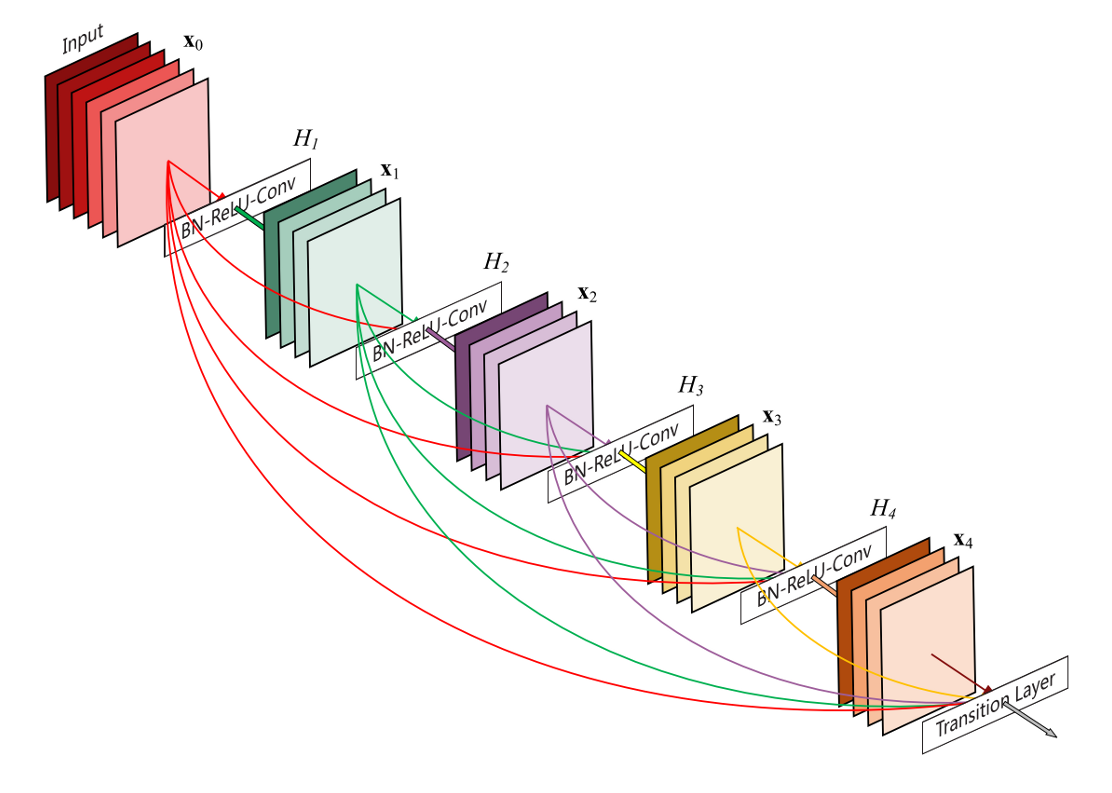
\includegraphics[width=.99\linewidth]{densenet.png} 
		\end{column}%
	\end{columns}
	\vfill %
	\footnotesize
	\color{blue} \url{https://arxiv.org/abs/1608.06993}
\end{frame}


\begin{frame}{Хотим компактности}
Нейросеть должна быть компактной и влезать на разные устройства (телефоны, IoT)

\begin{center}
	\begin{tabular}{|c|c|c|}
		\hline
	     Год & Архитектура & Примерный вес  \\ 
		\hline 
		2012 & AlexNet & 240 MB  \\ 
		\hline 
		2014 & VGG-19 & 549 MB  \\ 
		\hline 
		2015 & ResNet-50  & 98 MB \\ 
		\hline 
		2015 & ResNet-152  & 232 MB \\ 
		\hline 
		2015 & Inception v3  & 92 MB \\ 
		\hline 
		2016 & Inception-Resnet  & 215 MB  \\ 
		\hline 
	\end{tabular} 
	
	\par \mbox{ } \par
	
	\alert{Хотелось бы 20 MB максимум} 
\end{center} 
\vfill %
\footnotesize Веса указаны примерно:
\color{blue} \url{https://habr.com/ru/company/mipt/blog/450732/}
\end{frame}


\begin{frame}{MobileNet  (2017)}
	\begin{columns}[T] %
		\begin{column}{.35\textwidth}
			\begin{wideitemize}
				\item Легкая архитектура для мобильных устройств
				\item Комбинирует depthwise и pointwise convolution
				\item Есть просадка по качеству, но сильно уменьшаются требования по времени и памяти 
			\end{wideitemize} 
		\end{column}%
		\hfill%
		\begin{column}{.65\textwidth}
			\centering 	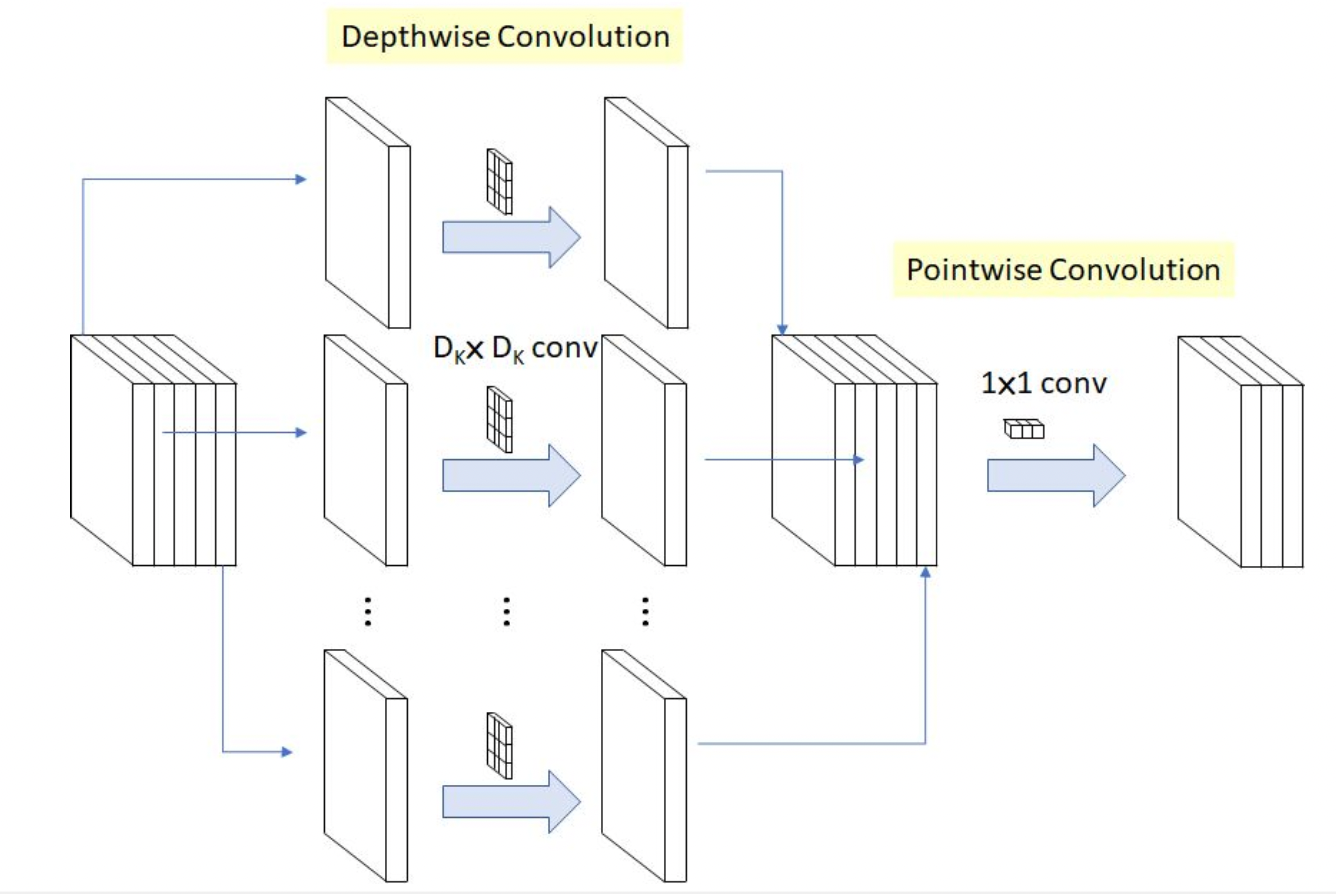
\includegraphics[width=.99\linewidth]{mobilenet.png} 
		\end{column}%
	\end{columns}
	\vfill %
	\footnotesize
	\color{blue} \url{https://arxiv.org/abs/1704.04861}
\end{frame}


% мб воткнуть NAS

\begin{frame}{Несвёрточные архитектуры}
		\begin{wideitemize}
			\item Текущие SOTA (state-of-the-art)  модели носят не свёрточные
			\item  Современные SOTA модели - трансформеры
			\item  Свёртки всё ещё часто используются, они быстрее работают и проще обучаются
			\item  Например, в январе 2022 вышла ConvNext, которая работает не хуже трансформера
		\end{wideitemize} 
\vfill %
\footnotesize
\color{blue} \url{https://arxiv.org/abs/2201.03545}
\end{frame}



\begin{transitionframe}
	\begin{center}
		\Huge История про Метрику
	\end{center}
\centering 
\includegraphics[scale = 0.7]{history_indi.jpg}
\end{transitionframe}


\begin{frame}{Метрика это кот}
\begin{center}
	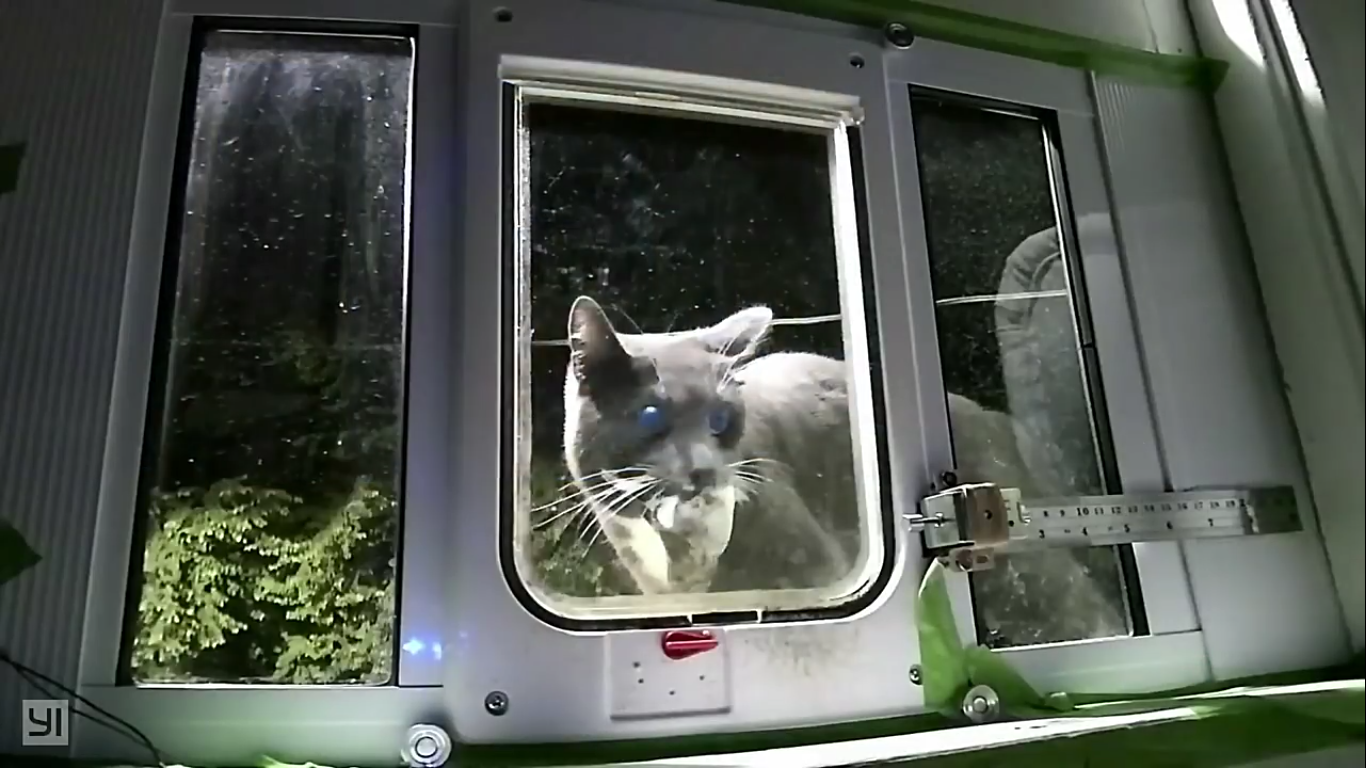
\includegraphics[width=.8\linewidth]{cat_metric1.png}
\end{center}
\vfill
\footnotesize
{\color{blue} \url{https://www.youtube.com/watch?v=1A-Nf3QIJjM}}
\end{frame}


\begin{frame}
\begin{center}
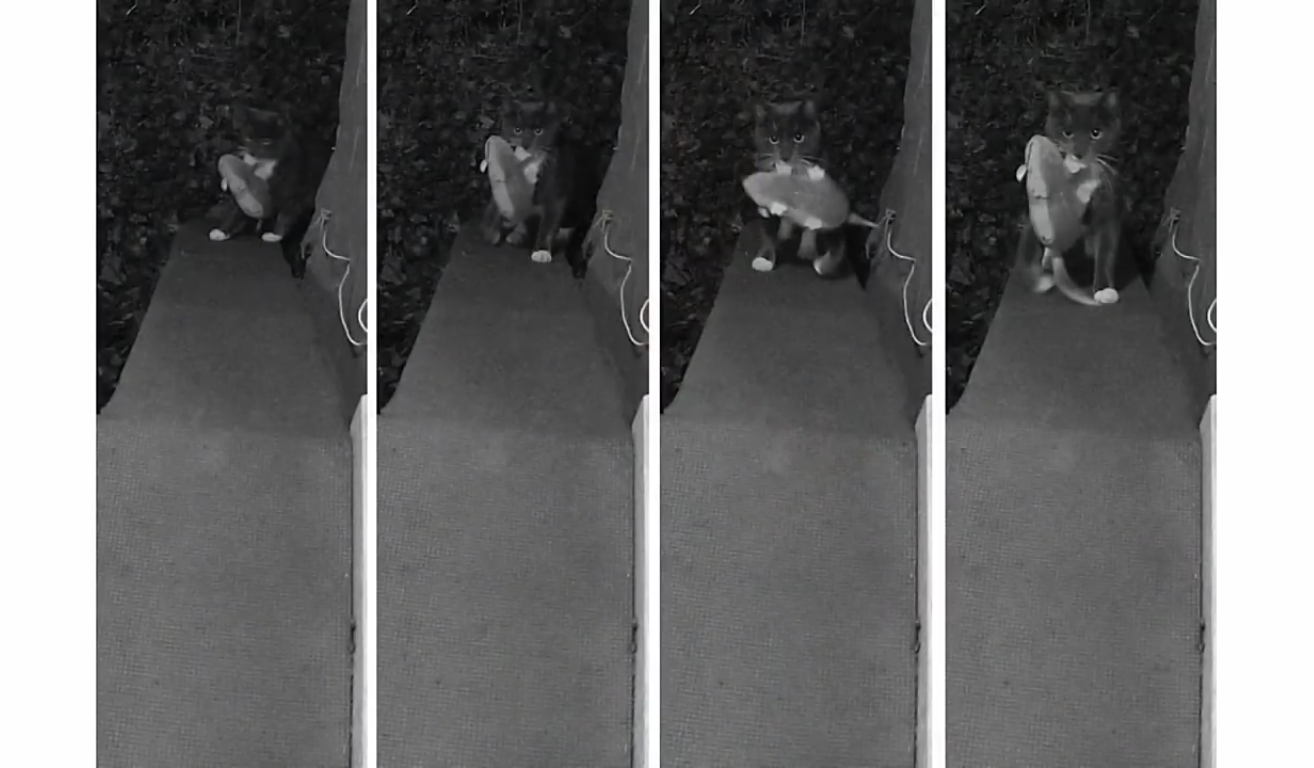
\includegraphics[width=.8\linewidth]{cat_metric2.png}
\end{center}
\end{frame}


\begin{frame}
\begin{center}
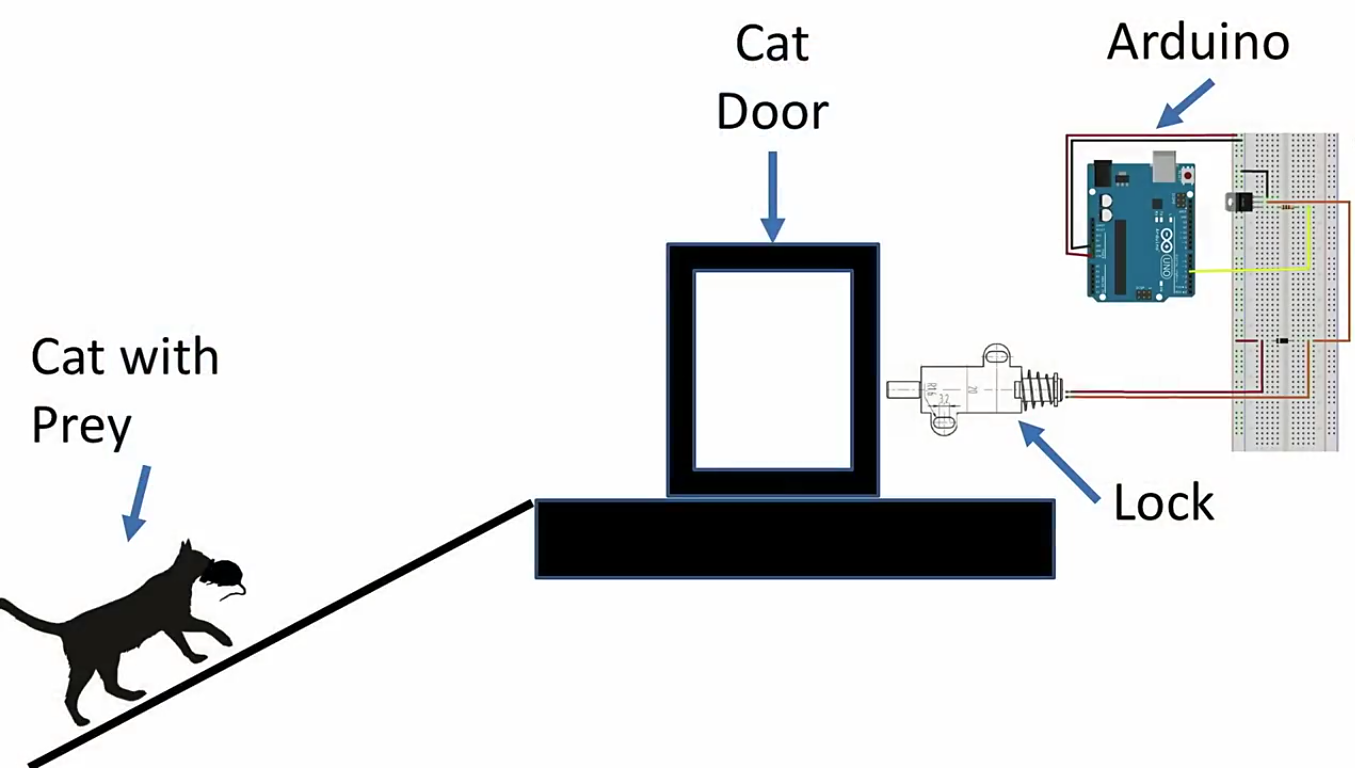
\includegraphics[width=.7\linewidth]{cat_metric3.png}
\end{center}
\end{frame}


\begin{frame}
\begin{center}
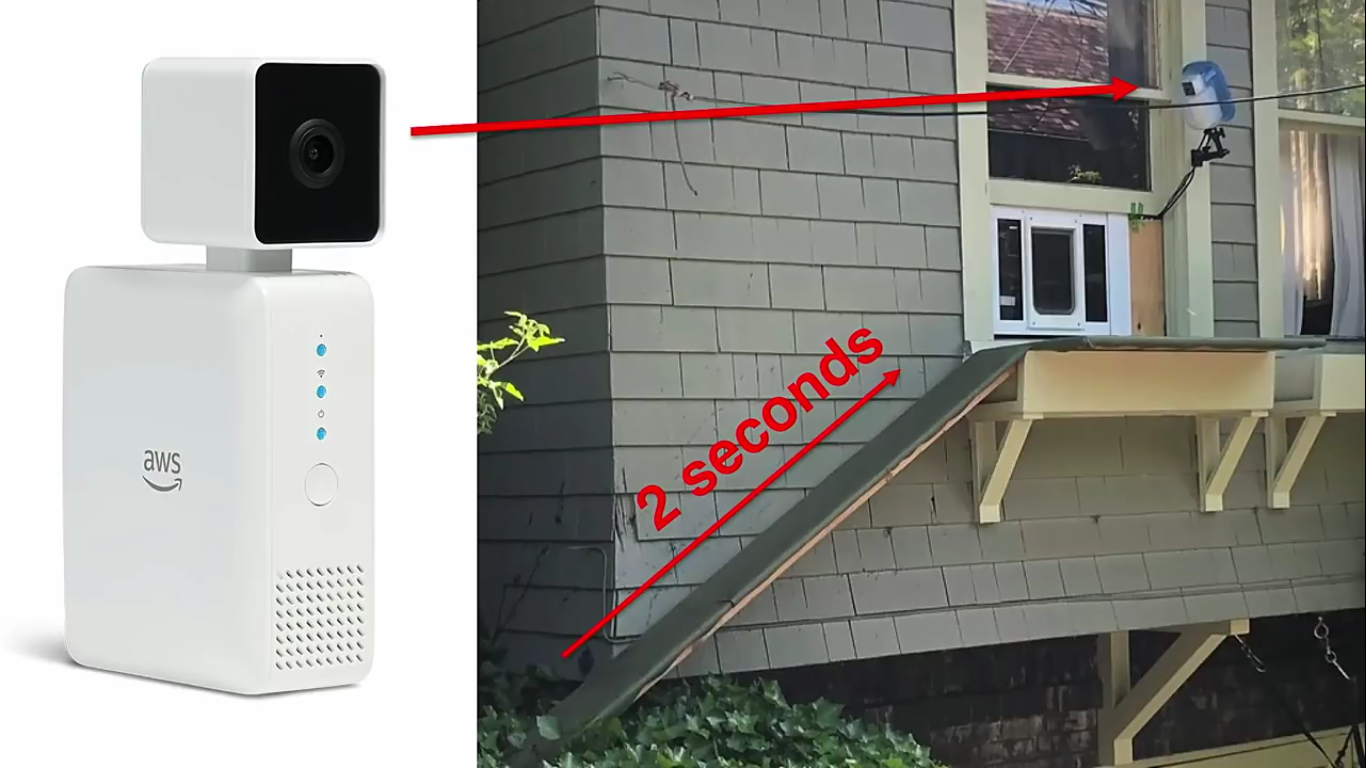
\includegraphics[width=.7\linewidth]{cat_metric4.png}
\end{center}
\end{frame}


\begin{frame}
\begin{center}
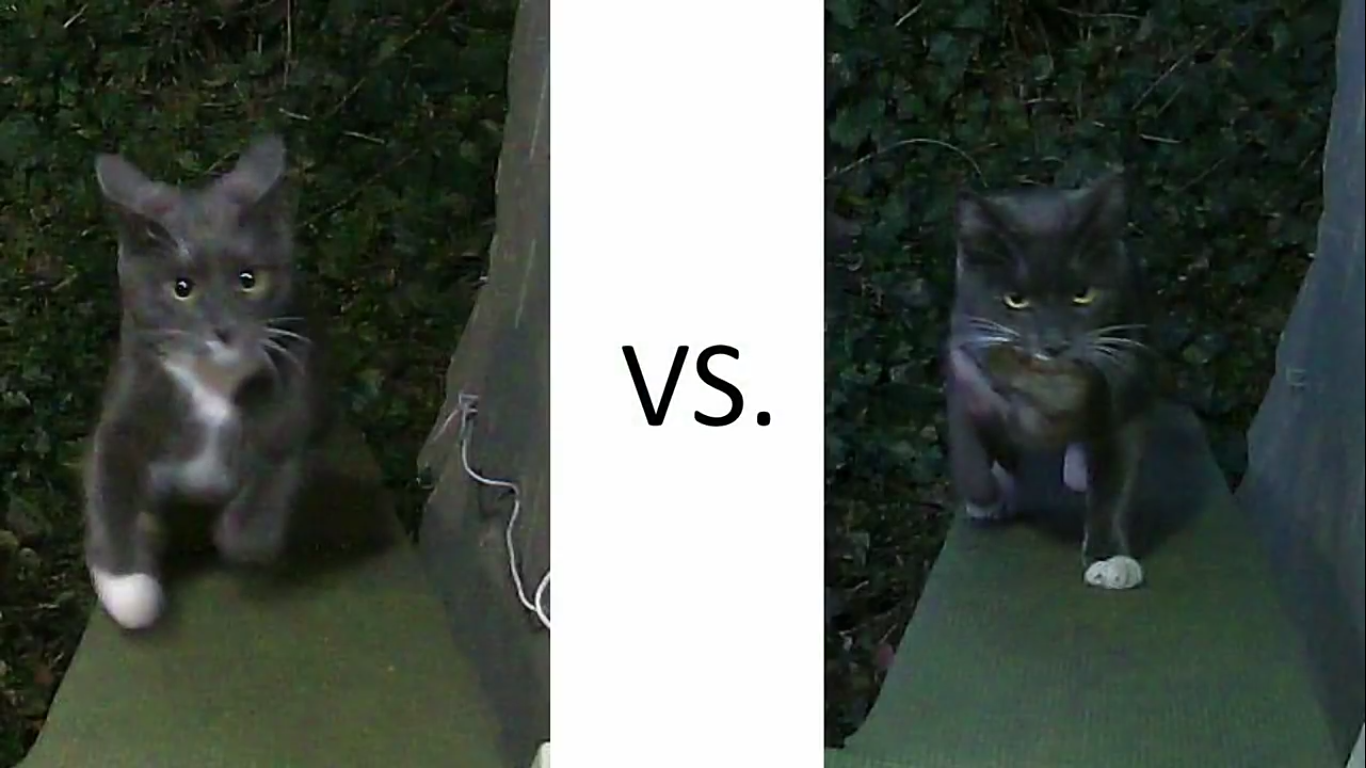
\includegraphics[width=.65\linewidth]{cat_metric5.png}
\end{center}
\end{frame}


\begin{frame}
\begin{center}
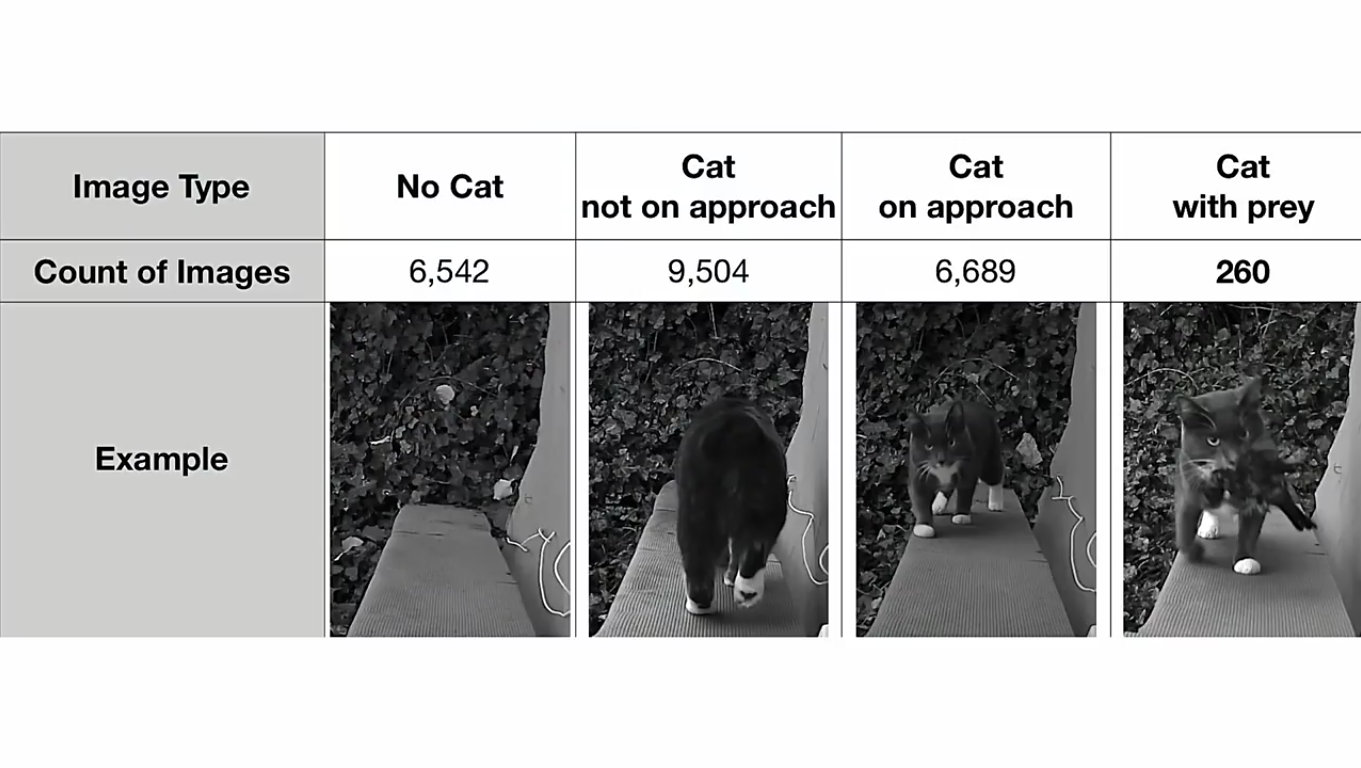
\includegraphics[width=.9\linewidth]{cat_metric6.png}
\end{center}
\end{frame}


\begin{frame}
\begin{center}
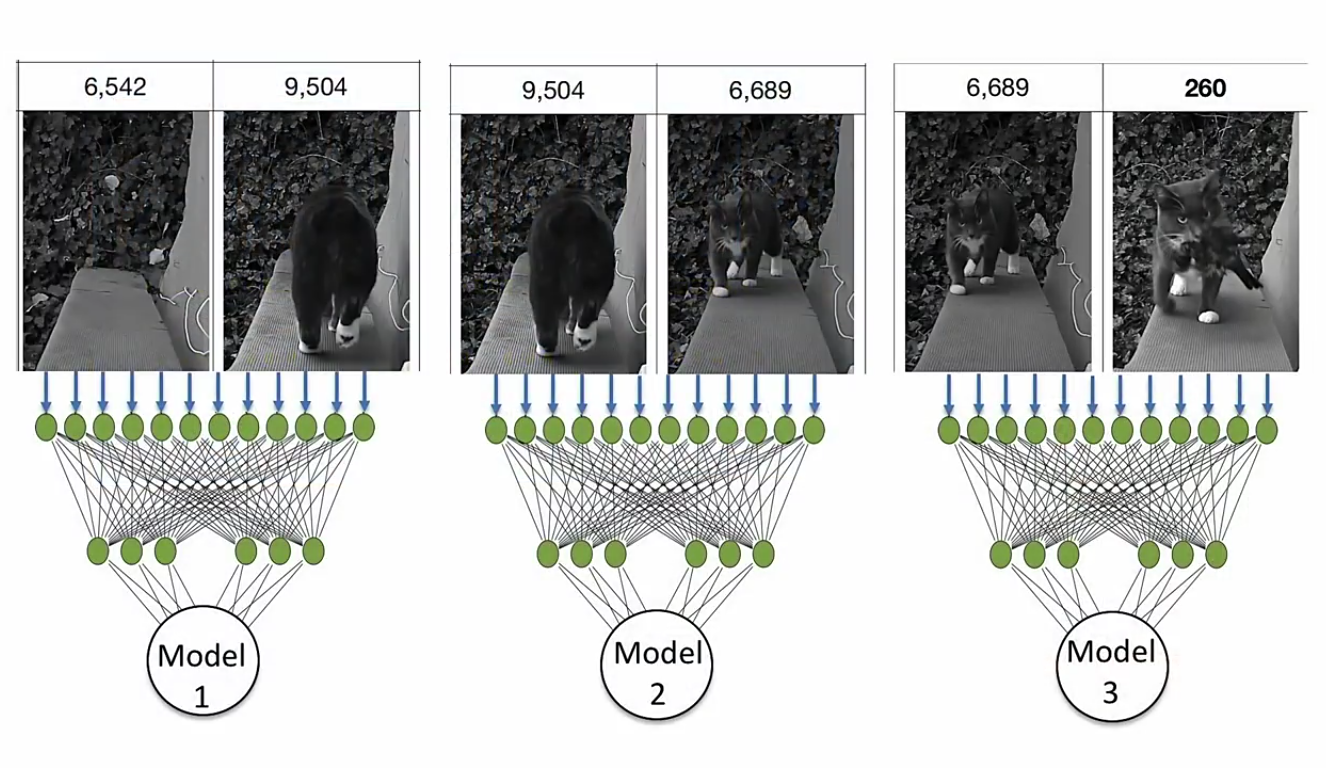
\includegraphics[width=.9\linewidth]{cat_metric7.png}
\end{center}
\end{frame}


\begin{frame}
\begin{center}
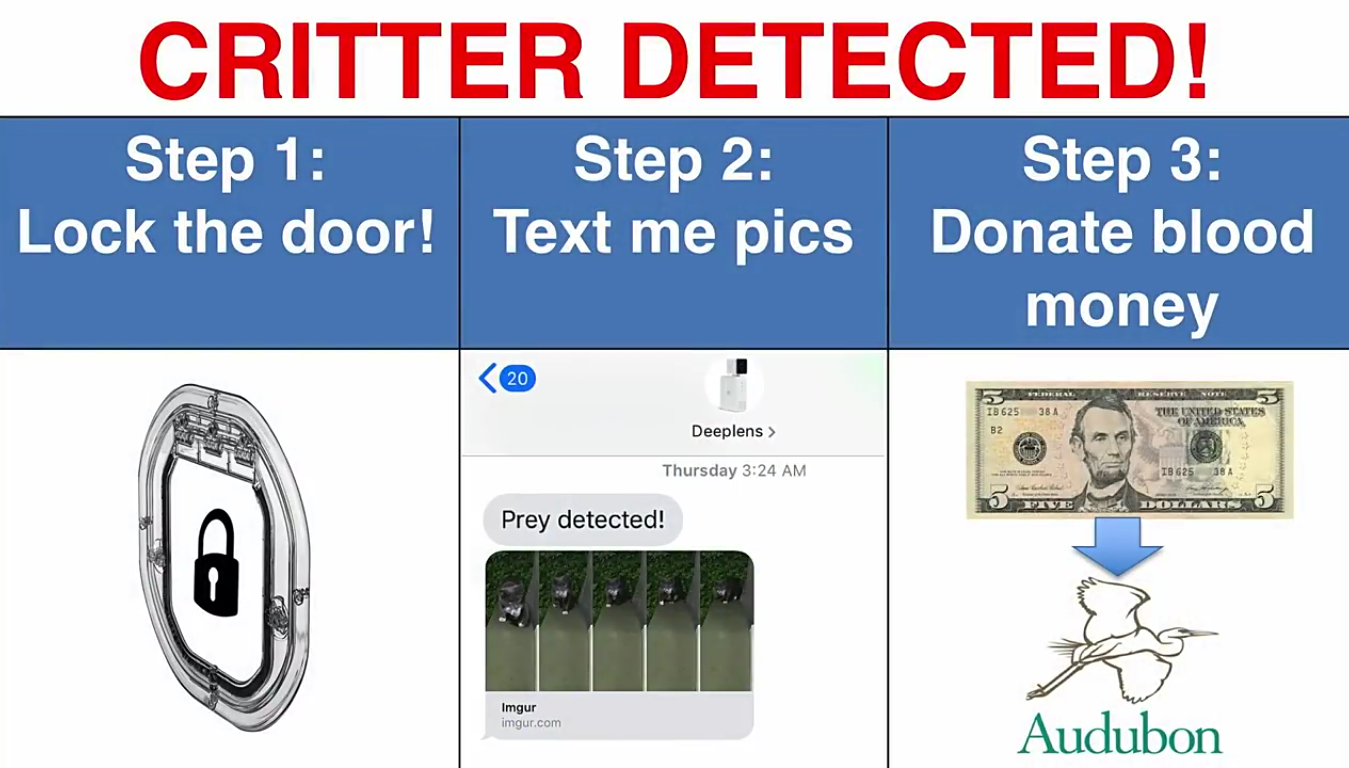
\includegraphics[width=.9\linewidth]{cat_metric9.png}
\end{center}
\end{frame}


\begin{frame}
\begin{center}
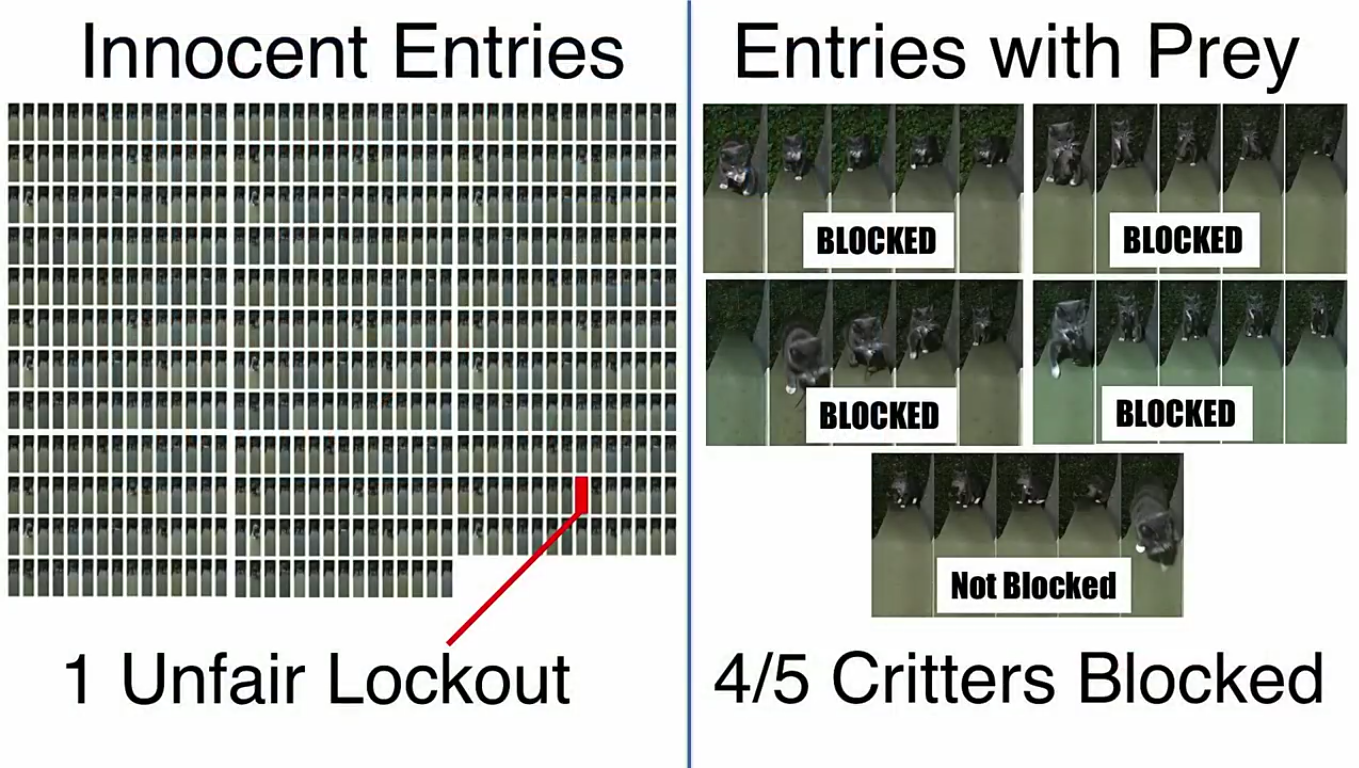
\includegraphics[width=.9\linewidth]{cat_metric8.png}
\end{center}
\end{frame}


\begin{frame}{Как он это сделал?}
\begin{wideitemize}
	\item   В выборке было всего лишь $260$ фотографий кота с добычей, неужели этого хватило для обучения сетки? 
	
	\item  На самом деле сетку с нуля никто не учил, делался \alert{transfer learning (перенос знаний)}
\end{wideitemize}
\end{frame}


\begin{transitionframe}
	\begin{center}
		\Huge Transfer learning (перенос знаний)
	\end{center}
\centering 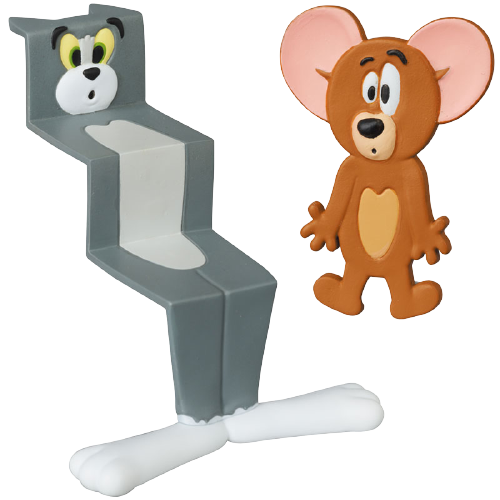
\includegraphics[scale = 0.2]{transfer_learning.png}
\end{transitionframe}


\begin{frame}{Transfer learning}
\begin{wideitemize}
	\item   На практике свёрточные сети с нуля обучают только большие технологические компании
	
	\item  Это происходит из-за ограниченности ресурсов
	
	\item  Уже обученные архитектуры пытаются адаптировать под новые задачи, это называется \alert{transfer learning (перенос знаний)}   
\end{wideitemize}
\end{frame}


\begin{frame}{Что выучивают нейросети}
\begin{center}
	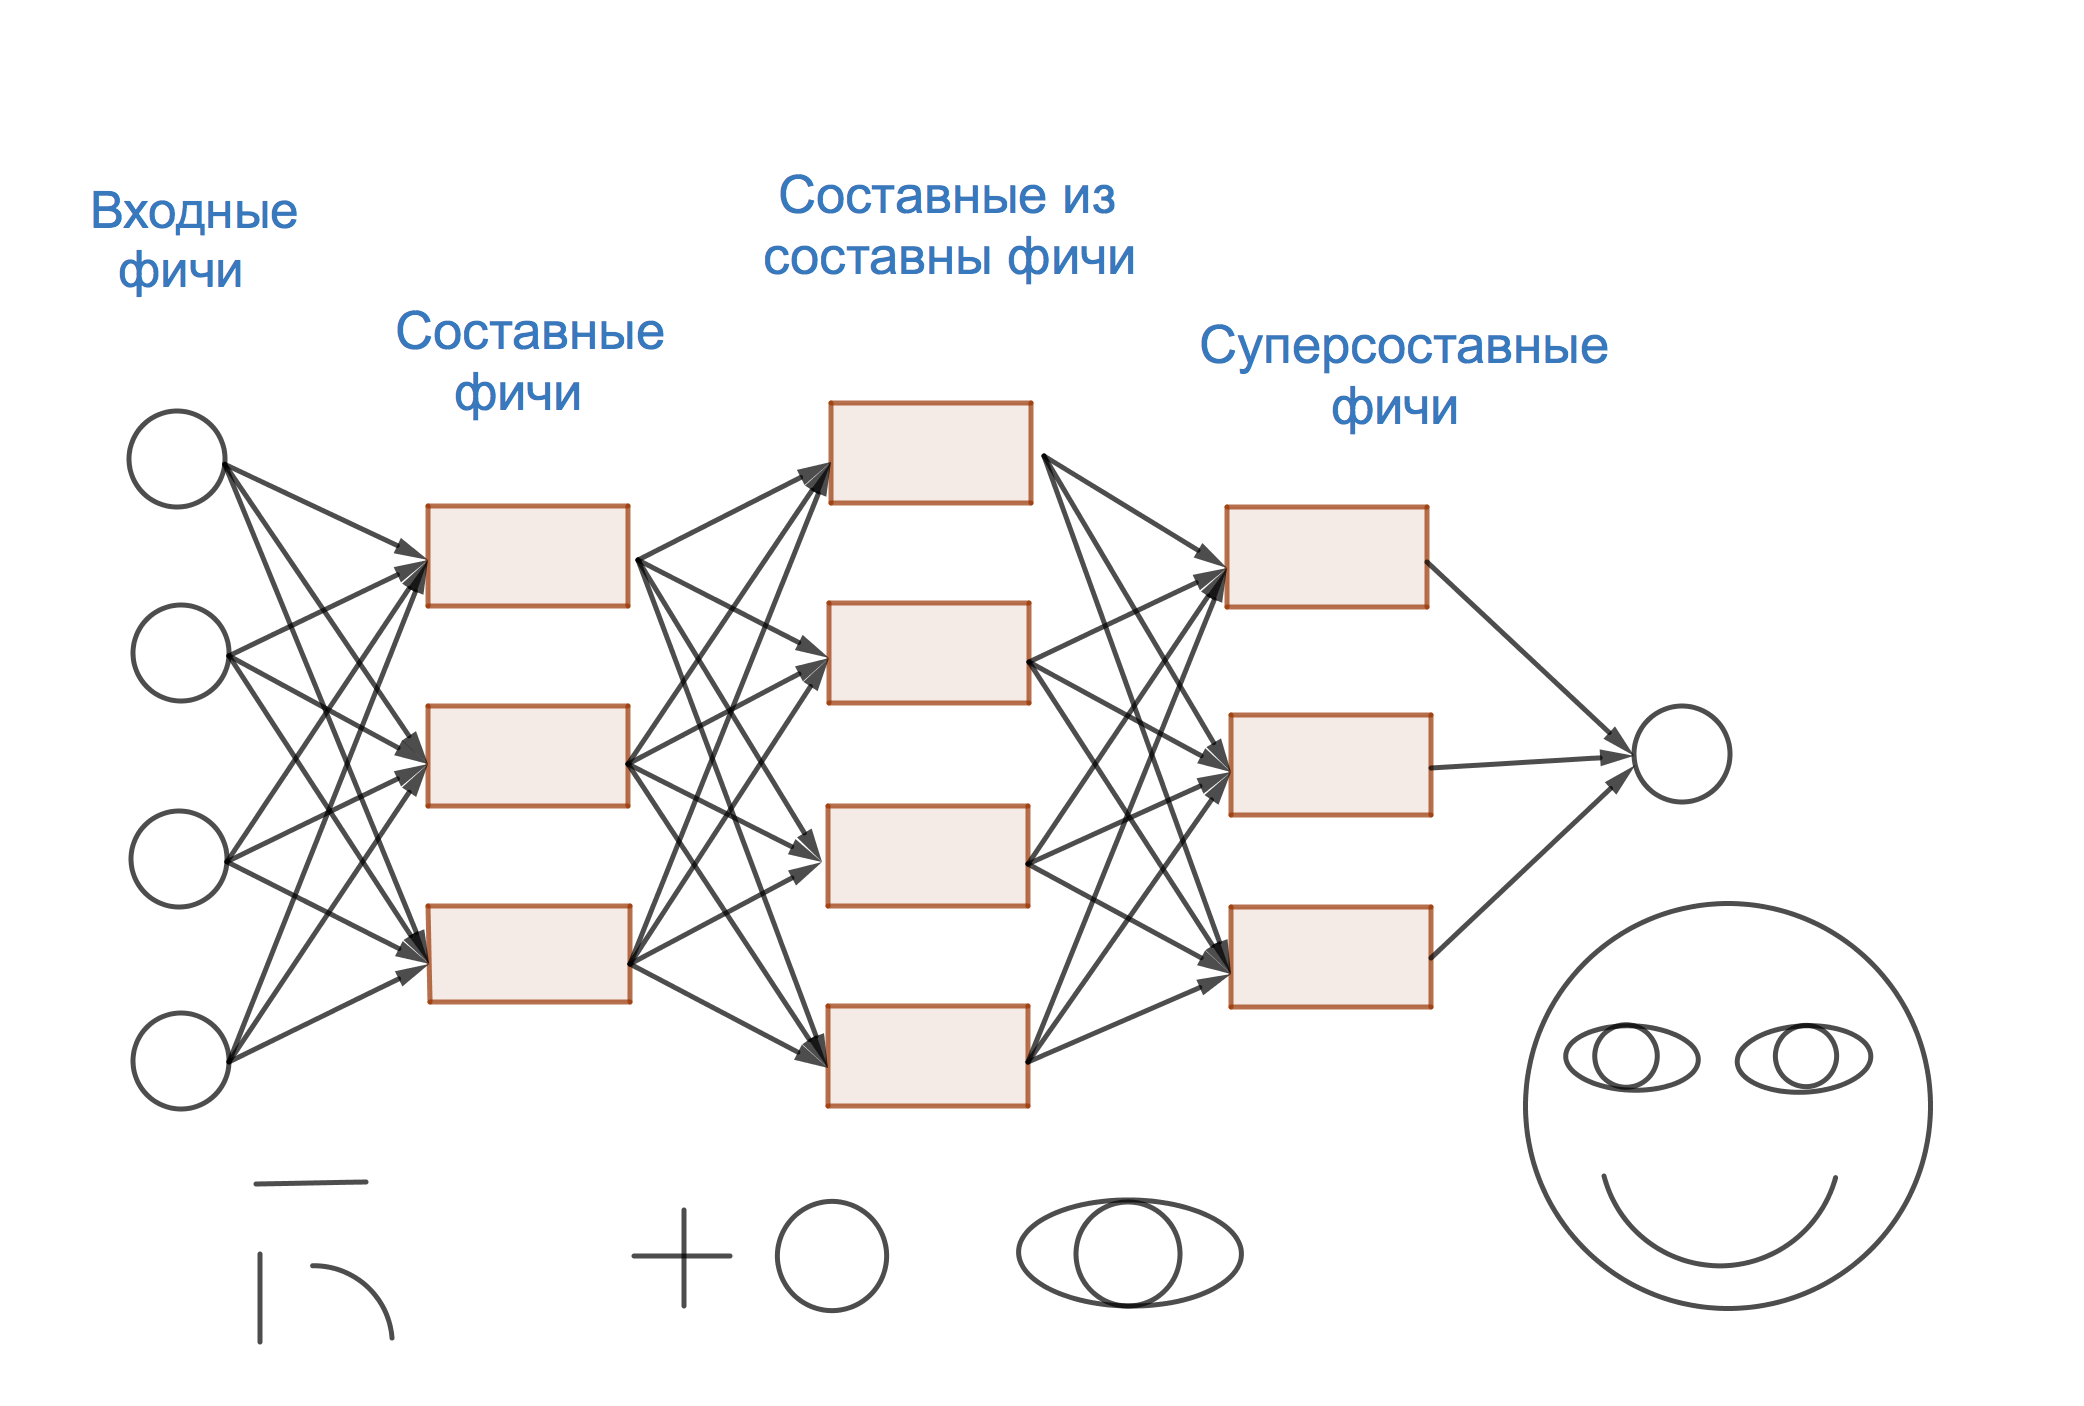
\includegraphics[width=0.73\paperwidth]{network_1.png}
\end{center}
\end{frame}


\begin{frame}{Transfer learning}
\begin{wideitemize}
\item  Глубокие сети извлекают из изображений сложные фичи, но для их обучения нужно много данных...
\only<2>{ \item  Давайте повторно использовать уже предобученную сеть! }
\end{wideitemize}

\only<1>{
	\begin{center}
		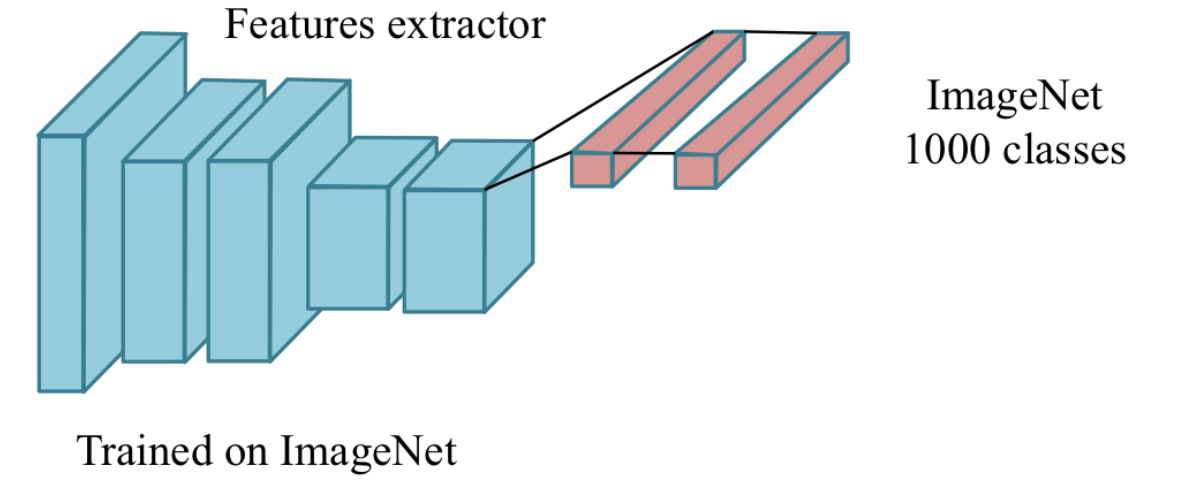
\includegraphics[width=.7\linewidth]{transfer_learning1.png}
	\end{center}
}

\only<2>{
	\begin{center}
	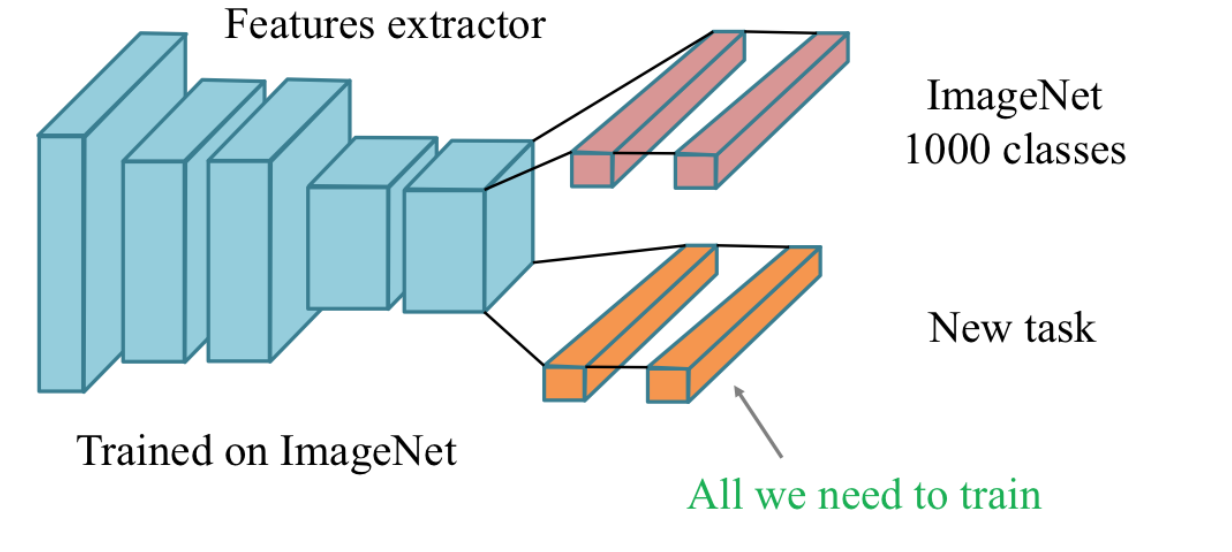
\includegraphics[width=.7\linewidth]{transfer_learning2.png}
	\end{center}
}
\end{frame}


\begin{frame}{Transfer learning}
\begin{wideitemize}
	\item  Нужно меньше данных для обучения, так как нас интересуют лишь последние слои
	\item  Как правило, на первых слоях фильтры похожие для всех задач
	\item  Чем сильнее новая задача отличается от исходной, тем больше слоёв нужно переучивать
	\item  Например, если мы хотим распознавать эмоции, в датасете для нашей сетки должны были быть человеческие лица
\end{wideitemize}
\end{frame}


\begin{frame}{Transfer learning}
\begin{center}
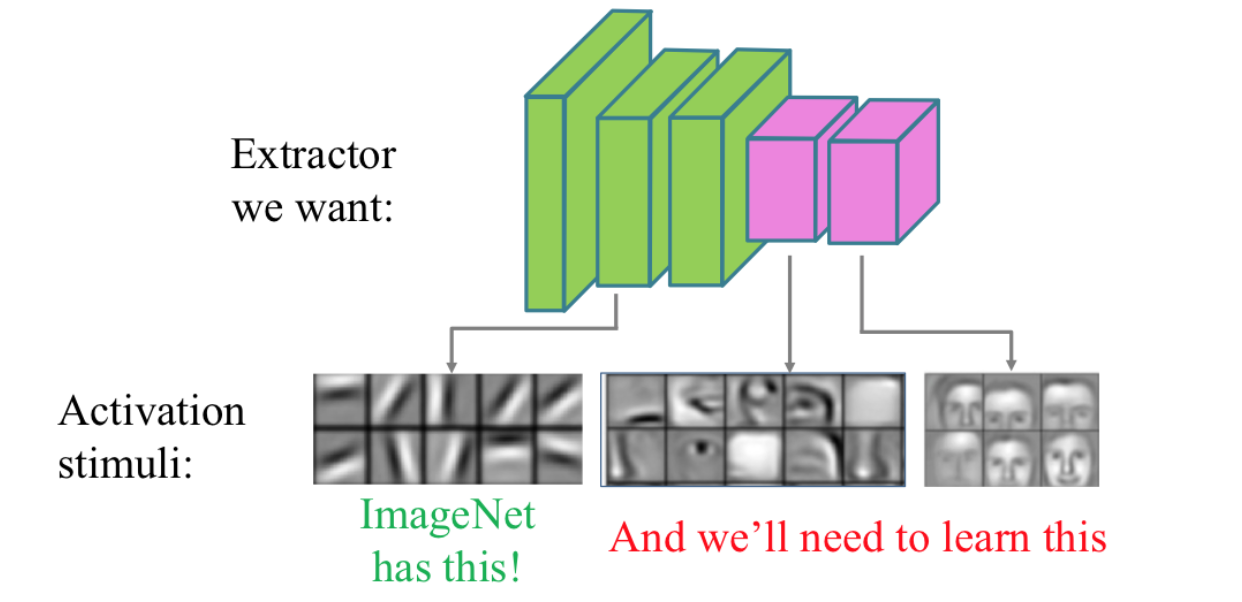
\includegraphics[width=.8\linewidth]{transfer_learning3.png}
\end{center}
\end{frame}


\begin{frame}{Transfer learning}
\begin{center}
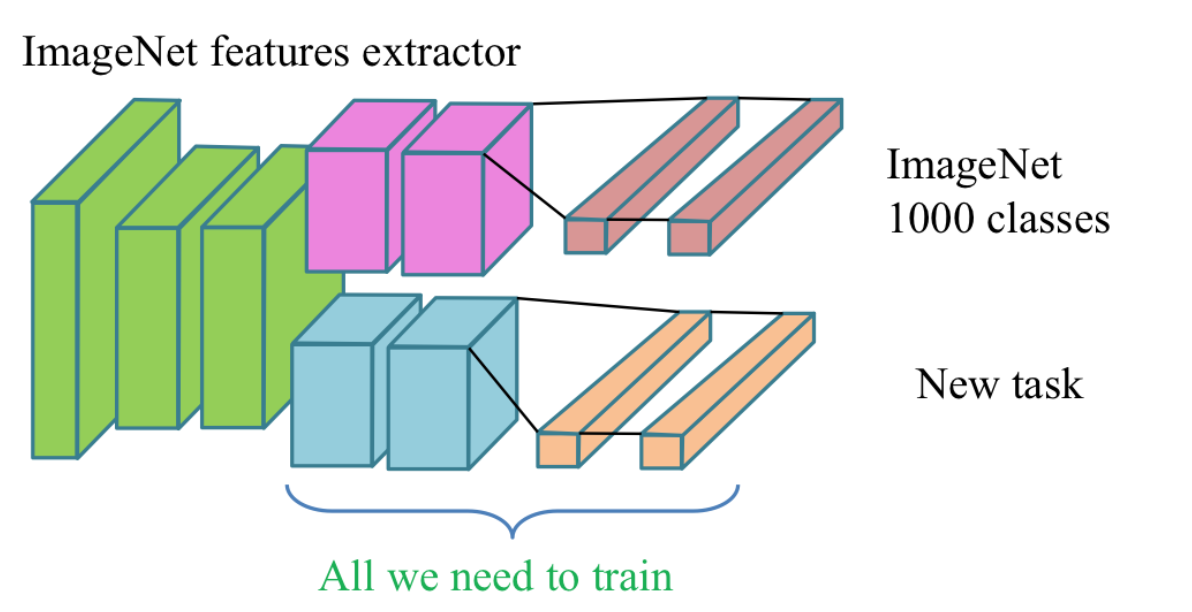
\includegraphics[width=.8\linewidth]{transfer_learning4.png}
\end{center}
\end{frame}


\begin{frame}{Finetuning}
\begin{wideitemize}
	\item  Можно инициализировать веса переучиваемых слоёв весами с ImageNet
	\item  Это называется \alert{finetuning,} так как инициализация неслучайная
\end{wideitemize}
\begin{center}
	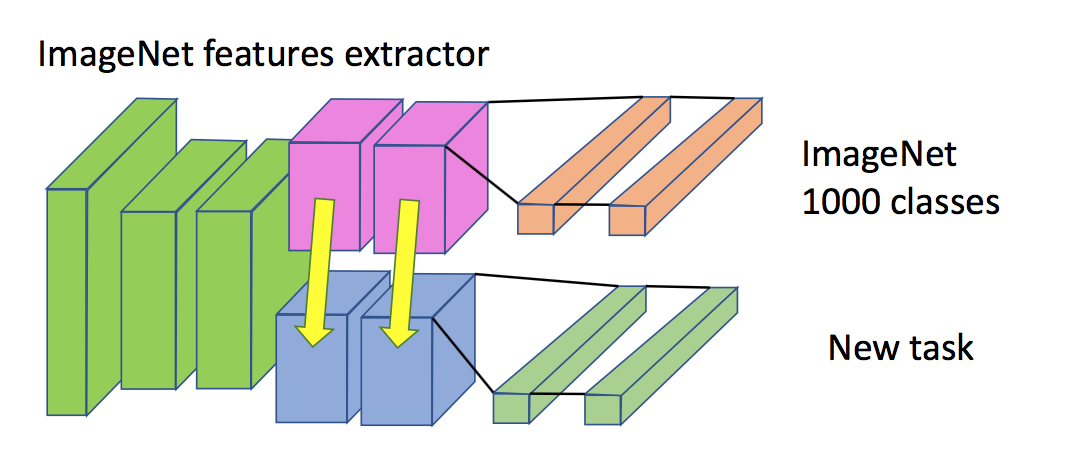
\includegraphics[width=.7\linewidth]{transfer_learning5.png}
\end{center}
\end{frame}


\begin{frame}{Ещё раз, ещё раз}
	\begin{columns}
	\begin{column}{0.33\textwidth}
		\alert{1. Обучаем на ImageNet}
		\begin{center}
			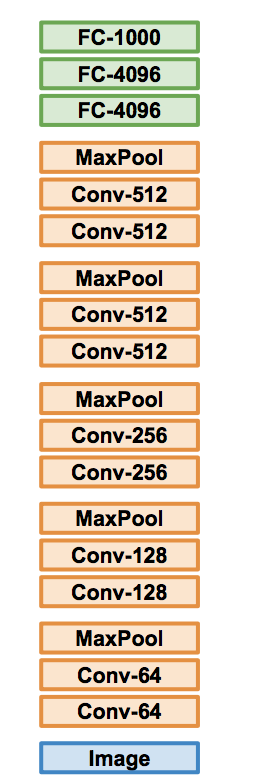
\includegraphics[width=.42\linewidth]{cs231_ft_1.png}
		\end{center}
	\end{column}
	\hfill
	\begin{column}{0.33\textwidth}
		\alert{2. Если задача похожа: transfer learning}
		\begin{center}
			\includegraphics[width=.82\linewidth]{cs231_ft_2.png}
		\end{center}
	\end{column}
	\hfill
	\begin{column}{0.33\textwidth}
		\alert{3. Задача немного отличается: finetuning}
		\begin{center}
			\includegraphics[width=.9\linewidth]{cs231_ft_3.png}
		\end{center}
	\end{column}
\end{columns}
\vfill %
\footnotesize
{\color{blue}  \url{http://cs231n.stanford.edu/slides/2021/}}
\end{frame}


\begin{frame}{Transfer learning}
	\begin{wideitemize}
		\item Чем больше датасет, тем больше слоёв можно доучивать
		\item При finetuning выставляйте более низкую скорость обучения
		\item Для начала попробуйте $0.1$ от оригинальной 
	\end{wideitemize}
\end{frame}


\begin{frame}{Transfer learning}
\begin{center}
	\includegraphics[width=.8\linewidth]{no_marginal.png}
	
\alert{Брать предобученные сети — нормальная, распространённая практика, а не маргинальные кейсы}
\end{center}
\vfill %
\footnotesize
{\color{blue}  \url{https://arxiv.org/pdf/1412.2306.pdf}}
\end{frame}


\begin{frame}{Transfer learning}
\begin{center}
	\includegraphics[width=.6\linewidth]{transfer_memes.png}
\end{center}
\end{frame}


%\begin{frame}{Зоопарки моделей}
%\begin{wideitemize}
%\item В интернете есть зоопарки с моделями
%\item  {\color{blue} \href{https://tfhub.dev/}{Зоопарк моделей внутри Tensorflow} }
%\item {\color{blue} \href{https://modelzoo.co/}{Другой большой зоопарк}}
%\item  {\color{blue}  \href{https://github.com/pytorch/vision}{Зоопарк для любителей pytorch}}
%\end{wideitemize}
%\end{frame}


%\begin{transitionframe}
%	\begin{center}
%		\Huge  Организация DL-экспериментов
%	\end{center}
%\end{transitionframe}
%
%
%\begin{frame}{Проблемы при обучении нейросетей}
%	\begin{wideitemize}
%		\item  «Neural net training is a leaky abstraction» — Andrej Karpathy
%		\item  Знания архитектур, оптимизаторов порой недостаточно для получения хорошей модели
%		\item Универсально наилучшего решения не бывает
%		\item Важна точка начала экспериментов и инкрементальные улучшения
%	\end{wideitemize}
%	\vfill
%	\footnotesize
%	{\color{blue} \url{http://karpathy.github.io/2019/04/25/recipe/} \newline Максим Рябинин: \url{https://github.com/aosokin/dl_cshse_ami/blob/master/2021-fall/lectures/DL21-fall-lecture5-bestpractices.pdf} }
%\end{frame}
%
%
%\begin{frame}{Перед началом}
%	\begin{wideitemize}
%		\item  Используйте проверенные временем стандарты
%		\item  Вместо своих моделей — архитектуры из популярных публикаций  (ResNet в зрении, ELMo/Transformer в текстах)
%		\item Adam со стандартным LR без расписания обойти нелегко
%		\item Сложные функции потерь/аугментации лучше отложить
%		\item Первые запуски на небольших датасетах, подвыборке или синтетике
%	\end{wideitemize}
%\end{frame}
%
%
%\begin{frame}{Как искать ошибки}
%	\begin{wideitemize}	
%		\item Чтобы легче находить ошибки, снизьте число факторов влияния 
%		
%		\item  Баги могут быть как в определении и обучении модели, так и в проверке качества (даже в загрузке данных)
%		
%		\item В меньшем масштабе можно быстрее итерироваться и находить проблемы
%		
%		\item \alert{Пробуйте прогнать код на одном батче и оценить, насколько адекватные результаты вы получили:} есть ли сходимость, есть ли переобучение на валидации, адекватно ли меняются метрики 
%		
%		\item Визуализируйте всё, что можете: метрики, примеры работы модели
%		
%		\item DL-код — всё ещё код: полезно писать unit-тесты
%	\end{wideitemize}
%\end{frame}
%
%
%
%\begin{frame}{Типичные ошибки: модели}
%	\begin{wideitemize}
%		\item Использование ad-hoc архитектур, когда не надо
%		\item Использование нестабильных/сложных функций потерь вместо кросс-энтропии в классификации 
%		\item Использование устаревших функций активации в глубоких сетях (сигмоид, тангенс)
%		\item Плохая инициализация: нули/константы вместо Glorot/He
%	\end{wideitemize}
%\end{frame}
%
%
%\begin{frame}{Типичные ошибки: данные}
%	\begin{wideitemize}
%		\item Отсутствие аугментации/использование некорректной аугментации, разные аугментации при обучении и валидации 
%		\item Если используете предобученные модели, препроцессинг данных должен быть максимально похожим 
%		\item Считывать все данные сразу, используйте Dataset 
%	\end{wideitemize}
%\end{frame}
%
%
%\begin{frame}{Типичные ошибки: обучение}
%	\begin{wideitemize}
%		\item Делайте чекпойнты, при них сохраняйте также параметры оптимизатора
%		\item Функция потерь должна быть максимально близка к метрике, которую вы оптимизируете 
%		\item Если используете pytorch, не забывайте делать \textit{zero\_grad} 
%	\end{wideitemize}
%\end{frame}
%
%
%% Посмотреть готовые инструменты для логов: 
%%  https://www.wandb.com/
%% [2] https://www.comet.ml/
%% [3] https://neptune.ai/ 
%\begin{frame}{Организация экспериментов}
%	\begin{wideitemize}
%		\item \alert{Тестируйте за один раз только одно изменение,} чтобы понимать влияние каждого фактора по отдельности 
%		\item На ранних стадиях не обязательно учить до сходимости и использовать всю выборку целиком
%		\item  Ведите лог всех экспериментов
%		\item Примеры инструментов для лога экспериентов:  \newline 
%		\url{https://www.wandb.com/}  \newline 
%		\url{https://www.comet.ml/}  \newline 
%		\url{https://neptune.ai/}  \newline 
%		\url{https://dvc.org/}  \newline 
%		\url{https://mlflow.org/}  \newline 
%	\end{wideitemize}
%	
%\end{frame}
%
%
%\begin{frame}{Как улучшать качество?}
%	\begin{wideitemize}
%		\item Функция потерь должна быть максимально близка к метрике
%		
%		\item  Начните с небольших экспериментов и масштабируйтесь, когда всё отлажено 
%		
%		\item  \alert{Работа с данными (количество, качество, предобработка) зачастую приносит гораздо больше эффекта, чем перебор архитектур и оптимизаторов}
%		
%		\item  Архитектуры влияют существенно, но учитывайте свои ресурсы
%		
%		\item Занимайтесь оптимизацией гиперпараметров в самую последнюю очередь 
%		
%		\item Размер батча важен (ряд моделей иначе просто не учится)

%	\end{wideitemize}
%\end{frame}
%
%
%\begin{frame}{Выводы}
%	\begin{wideitemize}
%		\item  Пользуйтесь проверенными техниками и опытом других людей
%		
%		\item  Начните с небольших экспериментов
%		
%		\item  Когда всё протестировано, можно масштабироваться
%		
%		\item  Отслеживайте все доступные метрики
%		
%		\item  Тестируйте одно изменение за раз
%		
%		\item  Сохраняйте код/конфигурацию всех экспериментов и их результаты
%		
%	\end{wideitemize}
%\end{frame}


\end{document}

